% Options for packages loaded elsewhere
\PassOptionsToPackage{unicode}{hyperref}
\PassOptionsToPackage{hyphens}{url}
%
\documentclass[
]{article}
\usepackage{lmodern}
\usepackage{amssymb,amsmath}
\usepackage{ifxetex,ifluatex}
\ifnum 0\ifxetex 1\fi\ifluatex 1\fi=0 % if pdftex
  \usepackage[T1]{fontenc}
  \usepackage[utf8]{inputenc}
  \usepackage{textcomp} % provide euro and other symbols
\else % if luatex or xetex
  \usepackage{unicode-math}
  \defaultfontfeatures{Scale=MatchLowercase}
  \defaultfontfeatures[\rmfamily]{Ligatures=TeX,Scale=1}
\fi
% Use upquote if available, for straight quotes in verbatim environments
\IfFileExists{upquote.sty}{\usepackage{upquote}}{}
\IfFileExists{microtype.sty}{% use microtype if available
  \usepackage[]{microtype}
  \UseMicrotypeSet[protrusion]{basicmath} % disable protrusion for tt fonts
}{}
\makeatletter
\@ifundefined{KOMAClassName}{% if non-KOMA class
  \IfFileExists{parskip.sty}{%
    \usepackage{parskip}
  }{% else
    \setlength{\parindent}{0pt}
    \setlength{\parskip}{6pt plus 2pt minus 1pt}}
}{% if KOMA class
  \KOMAoptions{parskip=half}}
\makeatother
\usepackage{xcolor}
\IfFileExists{xurl.sty}{\usepackage{xurl}}{} % add URL line breaks if available
\IfFileExists{bookmark.sty}{\usepackage{bookmark}}{\usepackage{hyperref}}
\hypersetup{
  pdftitle={Theoretical model},
  hidelinks,
  pdfcreator={LaTeX via pandoc}}
\urlstyle{same} % disable monospaced font for URLs
\usepackage[margin=1in]{geometry}
\usepackage{color}
\usepackage{fancyvrb}
\newcommand{\VerbBar}{|}
\newcommand{\VERB}{\Verb[commandchars=\\\{\}]}
\DefineVerbatimEnvironment{Highlighting}{Verbatim}{commandchars=\\\{\}}
% Add ',fontsize=\small' for more characters per line
\usepackage{framed}
\definecolor{shadecolor}{RGB}{248,248,248}
\newenvironment{Shaded}{\begin{snugshade}}{\end{snugshade}}
\newcommand{\AlertTok}[1]{\textcolor[rgb]{0.94,0.16,0.16}{#1}}
\newcommand{\AnnotationTok}[1]{\textcolor[rgb]{0.56,0.35,0.01}{\textbf{\textit{#1}}}}
\newcommand{\AttributeTok}[1]{\textcolor[rgb]{0.77,0.63,0.00}{#1}}
\newcommand{\BaseNTok}[1]{\textcolor[rgb]{0.00,0.00,0.81}{#1}}
\newcommand{\BuiltInTok}[1]{#1}
\newcommand{\CharTok}[1]{\textcolor[rgb]{0.31,0.60,0.02}{#1}}
\newcommand{\CommentTok}[1]{\textcolor[rgb]{0.56,0.35,0.01}{\textit{#1}}}
\newcommand{\CommentVarTok}[1]{\textcolor[rgb]{0.56,0.35,0.01}{\textbf{\textit{#1}}}}
\newcommand{\ConstantTok}[1]{\textcolor[rgb]{0.00,0.00,0.00}{#1}}
\newcommand{\ControlFlowTok}[1]{\textcolor[rgb]{0.13,0.29,0.53}{\textbf{#1}}}
\newcommand{\DataTypeTok}[1]{\textcolor[rgb]{0.13,0.29,0.53}{#1}}
\newcommand{\DecValTok}[1]{\textcolor[rgb]{0.00,0.00,0.81}{#1}}
\newcommand{\DocumentationTok}[1]{\textcolor[rgb]{0.56,0.35,0.01}{\textbf{\textit{#1}}}}
\newcommand{\ErrorTok}[1]{\textcolor[rgb]{0.64,0.00,0.00}{\textbf{#1}}}
\newcommand{\ExtensionTok}[1]{#1}
\newcommand{\FloatTok}[1]{\textcolor[rgb]{0.00,0.00,0.81}{#1}}
\newcommand{\FunctionTok}[1]{\textcolor[rgb]{0.00,0.00,0.00}{#1}}
\newcommand{\ImportTok}[1]{#1}
\newcommand{\InformationTok}[1]{\textcolor[rgb]{0.56,0.35,0.01}{\textbf{\textit{#1}}}}
\newcommand{\KeywordTok}[1]{\textcolor[rgb]{0.13,0.29,0.53}{\textbf{#1}}}
\newcommand{\NormalTok}[1]{#1}
\newcommand{\OperatorTok}[1]{\textcolor[rgb]{0.81,0.36,0.00}{\textbf{#1}}}
\newcommand{\OtherTok}[1]{\textcolor[rgb]{0.56,0.35,0.01}{#1}}
\newcommand{\PreprocessorTok}[1]{\textcolor[rgb]{0.56,0.35,0.01}{\textit{#1}}}
\newcommand{\RegionMarkerTok}[1]{#1}
\newcommand{\SpecialCharTok}[1]{\textcolor[rgb]{0.00,0.00,0.00}{#1}}
\newcommand{\SpecialStringTok}[1]{\textcolor[rgb]{0.31,0.60,0.02}{#1}}
\newcommand{\StringTok}[1]{\textcolor[rgb]{0.31,0.60,0.02}{#1}}
\newcommand{\VariableTok}[1]{\textcolor[rgb]{0.00,0.00,0.00}{#1}}
\newcommand{\VerbatimStringTok}[1]{\textcolor[rgb]{0.31,0.60,0.02}{#1}}
\newcommand{\WarningTok}[1]{\textcolor[rgb]{0.56,0.35,0.01}{\textbf{\textit{#1}}}}
\usepackage{graphicx,grffile}
\makeatletter
\def\maxwidth{\ifdim\Gin@nat@width>\linewidth\linewidth\else\Gin@nat@width\fi}
\def\maxheight{\ifdim\Gin@nat@height>\textheight\textheight\else\Gin@nat@height\fi}
\makeatother
% Scale images if necessary, so that they will not overflow the page
% margins by default, and it is still possible to overwrite the defaults
% using explicit options in \includegraphics[width, height, ...]{}
\setkeys{Gin}{width=\maxwidth,height=\maxheight,keepaspectratio}
% Set default figure placement to htbp
\makeatletter
\def\fps@figure{htbp}
\makeatother
\setlength{\emergencystretch}{3em} % prevent overfull lines
\providecommand{\tightlist}{%
  \setlength{\itemsep}{0pt}\setlength{\parskip}{0pt}}
\setcounter{secnumdepth}{-\maxdimen} % remove section numbering
\usepackage{booktabs}
\usepackage{longtable}
\usepackage{array}
\usepackage{multirow}
\usepackage{wrapfig}
\usepackage{float}
\usepackage{colortbl}
\usepackage{pdflscape}
\usepackage{tabu}
\usepackage{threeparttable}
\usepackage{threeparttablex}
\usepackage[normalem]{ulem}
\usepackage{makecell}
\usepackage{xcolor}

\title{Theoretical model}
\author{}
\date{\vspace{-2.5em}}

\begin{document}
\maketitle

Intraspecific variability is often seen as an unstructured, intrinsic
property of individuals, mostly genetic. Here, we rather investigate the
effect of spatial variations of the environment on individuals. Our
hypothesis is that the individuals can be clones, i.e.~have no genetic
differences, and still have different responses because the environment
in which they strive varies. As the response of an individual is a
result of all the environmental conditions it has encountered during its
life, the individual level is a tool to describe the environment more
acutely. This tool may incorporate some genetic differences, but is not
able to discriminate the genetic effect from the effect of local
environmental variation, or microsite effect. Moreover, the differences
between individuals due to environmental variation does not imply a
broader overlap of the species niches. Therefore, this type of
intraspecific variability has no effect on species coexistence directly.

We designed and conducted a virtual experiment that aims at illustrating
that intraspecific variability, or ``individual effects'', can result
from unobserved variation in some environmental variables
{[}@clark\_resolving\_2007{]}, therefore accounting for multidimensional
species differences which cannot be observed on a few niche axes.

To do so, we first consider a model that depicts the response of a
process, e.g.~growth, for individual clones of two different species to
all the environmental variables that influence it. Henceforth denoted
the ``Perfect knowledge model'', it represents the perfect knowledge of
the process as it occurs in the field and thus includes no residuals :

\(Y_{i,j,t} = \beta_{0,i} + \beta_{1,i} * X1_{i,j,t} + \ldots + \beta_{10,i} * X10_{i,j,t}\)
\hfill``Perfect knowledge model''

where \(1 \leq i \leq 2\) are the species ; \(1 \leq j \leq 500\) are
the individuals ; \(Y\) is a response variable, for instance growth ;
\(X1\) to \(X10\) are explanatory variables, for instance environmental
variables, that can vary with time \(t\) ; and the \(\beta_{k,i}\) ,
\(1 \leq k \leq 10\) depict the species-specific responses to these
environmental variables. As we consider clones, individuals of the same
species respond the same way to environmental variables, and variation
in \(Y\) among individuals within species is due to differences in the
environment where each individual thrives.

\begin{Shaded}
\begin{Highlighting}[]
\NormalTok{dim1 <-}\StringTok{ }\DecValTok{500}  \CommentTok{#dimension of the grid}
\NormalTok{dim2 <-}\StringTok{ }\DecValTok{500}
\NormalTok{nsp <-}\StringTok{ }\DecValTok{2}  \CommentTok{#number of species}
\NormalTok{nind <-}\StringTok{ }\DecValTok{500}  \CommentTok{#number of individuals per species}
\NormalTok{ntime <-}\StringTok{ }\DecValTok{2}  \CommentTok{#number of observations per individual}
\NormalTok{nobs <-}\StringTok{ }\NormalTok{nsp }\OperatorTok{*}\StringTok{ }\NormalTok{nind }\OperatorTok{*}\StringTok{ }\NormalTok{ntime  }\CommentTok{#number of observations}
\end{Highlighting}
\end{Shaded}

\begin{Shaded}
\begin{Highlighting}[]
\CommentTok{# 10 parameters of species 1 and 2 To modulate the overlap of}
\CommentTok{# the growth of both species, use the 9 random parameters :}
\CommentTok{# the closer to the second parameter, the more confused the}
\CommentTok{# statistical model will be. If many parameters are negative,}
\CommentTok{# it can even lead to a negative mean G ~ L relationship. In}
\CommentTok{# the current code, 5 variables have a positive effect on}
\CommentTok{# growth and 4 a negative effect.}

\NormalTok{param1 =}\StringTok{ }\KeywordTok{c}\NormalTok{(}\FloatTok{0.25}\NormalTok{, }\FloatTok{0.15}\NormalTok{, }\KeywordTok{abs}\NormalTok{(}\KeywordTok{runif}\NormalTok{(}\DecValTok{5}\NormalTok{, }\FloatTok{-0.05}\NormalTok{, }\FloatTok{0.05}\NormalTok{)), }\OperatorTok{-}\KeywordTok{abs}\NormalTok{(}\KeywordTok{runif}\NormalTok{(}\DecValTok{4}\NormalTok{, }
    \FloatTok{-0.05}\NormalTok{, }\FloatTok{0.05}\NormalTok{)))}
\NormalTok{param2 =}\StringTok{ }\KeywordTok{c}\NormalTok{(}\FloatTok{0.2}\NormalTok{, }\FloatTok{0.1}\NormalTok{, }\KeywordTok{abs}\NormalTok{(}\KeywordTok{runif}\NormalTok{(}\DecValTok{5}\NormalTok{, }\FloatTok{-0.05}\NormalTok{, }\FloatTok{0.05}\NormalTok{)), }\OperatorTok{-}\KeywordTok{abs}\NormalTok{(}\KeywordTok{runif}\NormalTok{(}\DecValTok{4}\NormalTok{, }
    \FloatTok{-0.05}\NormalTok{, }\FloatTok{0.05}\NormalTok{)))}

\NormalTok{par_sp <-}\StringTok{ }\KeywordTok{cbind}\NormalTok{(param1, param2)}

\CommentTok{# Adding genetic IV}
\NormalTok{par_ind1 <-}\StringTok{ }\KeywordTok{rbind}\NormalTok{(}\KeywordTok{rnorm}\NormalTok{(nind, param1[}\DecValTok{1}\NormalTok{], }\KeywordTok{abs}\NormalTok{(param1[}\DecValTok{1}\NormalTok{]}\OperatorTok{/}\DecValTok{4}\NormalTok{)), }\KeywordTok{rnorm}\NormalTok{(nind, }
\NormalTok{    param1[}\DecValTok{2}\NormalTok{], }\KeywordTok{abs}\NormalTok{(param1[}\DecValTok{2}\NormalTok{]}\OperatorTok{/}\DecValTok{4}\NormalTok{)), }\KeywordTok{rnorm}\NormalTok{(nind, param1[}\DecValTok{3}\NormalTok{], }\KeywordTok{abs}\NormalTok{(param1[}\DecValTok{3}\NormalTok{]}\OperatorTok{/}\DecValTok{4}\NormalTok{)), }
    \KeywordTok{rnorm}\NormalTok{(nind, param1[}\DecValTok{4}\NormalTok{], }\KeywordTok{abs}\NormalTok{(param1[}\DecValTok{4}\NormalTok{]}\OperatorTok{/}\DecValTok{4}\NormalTok{)), }\KeywordTok{rnorm}\NormalTok{(nind, param1[}\DecValTok{5}\NormalTok{], }
        \KeywordTok{abs}\NormalTok{(param1[}\DecValTok{5}\NormalTok{]}\OperatorTok{/}\DecValTok{4}\NormalTok{)), }\KeywordTok{rnorm}\NormalTok{(nind, param1[}\DecValTok{6}\NormalTok{], }\KeywordTok{abs}\NormalTok{(param1[}\DecValTok{6}\NormalTok{]}\OperatorTok{/}\DecValTok{4}\NormalTok{)), }
    \KeywordTok{rnorm}\NormalTok{(nind, param1[}\DecValTok{7}\NormalTok{], }\KeywordTok{abs}\NormalTok{(param1[}\DecValTok{7}\NormalTok{]}\OperatorTok{/}\DecValTok{4}\NormalTok{)), }\KeywordTok{rnorm}\NormalTok{(nind, param1[}\DecValTok{8}\NormalTok{], }
        \KeywordTok{abs}\NormalTok{(param1[}\DecValTok{8}\NormalTok{]}\OperatorTok{/}\DecValTok{4}\NormalTok{)), }\KeywordTok{rnorm}\NormalTok{(nind, param1[}\DecValTok{9}\NormalTok{], }\KeywordTok{abs}\NormalTok{(param1[}\DecValTok{9}\NormalTok{]}\OperatorTok{/}\DecValTok{4}\NormalTok{)), }
    \KeywordTok{rnorm}\NormalTok{(nind, param1[}\DecValTok{10}\NormalTok{], }\KeywordTok{abs}\NormalTok{(param1[}\DecValTok{10}\NormalTok{]}\OperatorTok{/}\DecValTok{4}\NormalTok{)), }\KeywordTok{rnorm}\NormalTok{(nind, param1[}\DecValTok{11}\NormalTok{], }
        \KeywordTok{abs}\NormalTok{(param1[}\DecValTok{11}\NormalTok{]}\OperatorTok{/}\DecValTok{4}\NormalTok{)))}
\NormalTok{par_ind2 <-}\StringTok{ }\KeywordTok{rbind}\NormalTok{(}\KeywordTok{rnorm}\NormalTok{(nind, param2[}\DecValTok{1}\NormalTok{], }\KeywordTok{abs}\NormalTok{(param2[}\DecValTok{1}\NormalTok{]}\OperatorTok{/}\DecValTok{4}\NormalTok{)), }\KeywordTok{rnorm}\NormalTok{(nind, }
\NormalTok{    param2[}\DecValTok{2}\NormalTok{], }\KeywordTok{abs}\NormalTok{(param2[}\DecValTok{2}\NormalTok{]}\OperatorTok{/}\DecValTok{4}\NormalTok{)), }\KeywordTok{rnorm}\NormalTok{(nind, param2[}\DecValTok{3}\NormalTok{], }\KeywordTok{abs}\NormalTok{(param2[}\DecValTok{3}\NormalTok{]}\OperatorTok{/}\DecValTok{4}\NormalTok{)), }
    \KeywordTok{rnorm}\NormalTok{(nind, param2[}\DecValTok{4}\NormalTok{], }\KeywordTok{abs}\NormalTok{(param2[}\DecValTok{4}\NormalTok{]}\OperatorTok{/}\DecValTok{4}\NormalTok{)), }\KeywordTok{rnorm}\NormalTok{(nind, param2[}\DecValTok{5}\NormalTok{], }
        \KeywordTok{abs}\NormalTok{(param2[}\DecValTok{5}\NormalTok{]}\OperatorTok{/}\DecValTok{4}\NormalTok{)), }\KeywordTok{rnorm}\NormalTok{(nind, param2[}\DecValTok{6}\NormalTok{], }\KeywordTok{abs}\NormalTok{(param2[}\DecValTok{6}\NormalTok{]}\OperatorTok{/}\DecValTok{4}\NormalTok{)), }
    \KeywordTok{rnorm}\NormalTok{(nind, param2[}\DecValTok{7}\NormalTok{], }\KeywordTok{abs}\NormalTok{(param2[}\DecValTok{7}\NormalTok{]}\OperatorTok{/}\DecValTok{4}\NormalTok{)), }\KeywordTok{rnorm}\NormalTok{(nind, param2[}\DecValTok{8}\NormalTok{], }
        \KeywordTok{abs}\NormalTok{(param2[}\DecValTok{8}\NormalTok{]}\OperatorTok{/}\DecValTok{4}\NormalTok{)), }\KeywordTok{rnorm}\NormalTok{(nind, param2[}\DecValTok{9}\NormalTok{], }\KeywordTok{abs}\NormalTok{(param2[}\DecValTok{9}\NormalTok{]}\OperatorTok{/}\DecValTok{4}\NormalTok{)), }
    \KeywordTok{rnorm}\NormalTok{(nind, param2[}\DecValTok{10}\NormalTok{], }\KeywordTok{abs}\NormalTok{(param2[}\DecValTok{10}\NormalTok{]}\OperatorTok{/}\DecValTok{4}\NormalTok{)), }\KeywordTok{rnorm}\NormalTok{(nind, param2[}\DecValTok{11}\NormalTok{], }
        \KeywordTok{abs}\NormalTok{(param2[}\DecValTok{11}\NormalTok{]}\OperatorTok{/}\DecValTok{4}\NormalTok{)))}
\NormalTok{par_ind <-}\StringTok{ }\KeywordTok{cbind}\NormalTok{(par_ind1, par_ind2)}
\end{Highlighting}
\end{Shaded}

We fix the species parameters of the ``Perfect knowledge model'' as
follows:

Parameters of species 1 : \(\beta_0\) = 0.25, \(\beta_1\) = 0.15,
\(\beta_2\) to \(\beta_{6}\) are chosen randomly between -0.05 and 0.05
and \(\beta_{7}\) to \(\beta_{10}\) are chosen randomly between 0 and
0.05.

Parameters of species 2 : \(\beta_0\) = 0.2, \(\beta_1\) = 0.1,
\(\beta_2\) to \(\beta_{10}\) are chosen the same way as for species 1.

The difference between the species is imposed by those parameters. Here,
the species 1 is more performant on average thanks to its higher
intercept (\(\beta_0\)) and reaction to the first environmental variable
(\(\beta_1\)). The first environmental variable (\(X1\)) has a higher
weight in the computation of the response variable, as would be light
for growth for instance.

To account for genetic variability in our generated data, we add an
intraspecific variability in species parameters by sampling each
individual parameter in a normal distribution centered on the species
mean parameter and with a standard deviation of a quarter of the species
mean parameter.

To represent the spatialised environment of such a forest plot, we build
a 2D matrix of dimension 500 \(\times\) 500 for each environmental
variable at a time \(t_0\), by randomly generating them with spatial
autocorrelation. We here consider that all environmental variables are
independent. Each variable is simulated by using the gstat package,
enabling to create autocorrelated random fields. A spherical
semivariogram model is used for each of the ten environmental variables,
with a mean of 0 for each explanatory variable (beta = 0), a sill of 1
(psill = 1) for each and a range of 50 (range = 50).

\begin{Shaded}
\begin{Highlighting}[]
\CommentTok{# Matrixes of variables Structure (coordinates)}
\NormalTok{xy <-}\StringTok{ }\KeywordTok{expand.grid}\NormalTok{(}\DecValTok{1}\OperatorTok{:}\NormalTok{dim1, }\DecValTok{1}\OperatorTok{:}\NormalTok{dim2)}
\KeywordTok{names}\NormalTok{(xy) <-}\StringTok{ }\KeywordTok{c}\NormalTok{(}\StringTok{"x"}\NormalTok{, }\StringTok{"y"}\NormalTok{)}

\CommentTok{# Spatial models}
\NormalTok{mods <-}\StringTok{ }\KeywordTok{list}\NormalTok{()}
\NormalTok{mods[[}\DecValTok{1}\NormalTok{]] <-}\StringTok{ }\NormalTok{gstat}\OperatorTok{::}\KeywordTok{gstat}\NormalTok{(}\DataTypeTok{formula =}\NormalTok{ z }\OperatorTok{~}\StringTok{ }\DecValTok{1}\NormalTok{, }\DataTypeTok{locations =} \OperatorTok{~}\NormalTok{x }\OperatorTok{+}\StringTok{ }\NormalTok{y, }
    \DataTypeTok{dummy =}\NormalTok{ T, }\DataTypeTok{beta =} \DecValTok{0}\NormalTok{, }\DataTypeTok{model =}\NormalTok{ gstat}\OperatorTok{::}\KeywordTok{vgm}\NormalTok{(}\DataTypeTok{psill =} \DecValTok{1}\NormalTok{, }\DataTypeTok{model =} \StringTok{"Sph"}\NormalTok{, }
        \DataTypeTok{range =} \DecValTok{50}\NormalTok{, }\DataTypeTok{nugget =} \DecValTok{0}\NormalTok{), }\DataTypeTok{nmax =} \DecValTok{20}\NormalTok{)}
\NormalTok{mods[[}\DecValTok{2}\NormalTok{]] <-}\StringTok{ }\NormalTok{gstat}\OperatorTok{::}\KeywordTok{gstat}\NormalTok{(}\DataTypeTok{formula =}\NormalTok{ z }\OperatorTok{~}\StringTok{ }\DecValTok{1}\NormalTok{, }\DataTypeTok{locations =} \OperatorTok{~}\NormalTok{x }\OperatorTok{+}\StringTok{ }\NormalTok{y, }
    \DataTypeTok{dummy =}\NormalTok{ T, }\DataTypeTok{beta =} \DecValTok{0}\NormalTok{, }\DataTypeTok{model =}\NormalTok{ gstat}\OperatorTok{::}\KeywordTok{vgm}\NormalTok{(}\DataTypeTok{psill =} \DecValTok{1}\NormalTok{, }\DataTypeTok{model =} \StringTok{"Sph"}\NormalTok{, }
        \DataTypeTok{range =} \DecValTok{50}\NormalTok{, }\DataTypeTok{nugget =} \DecValTok{0}\NormalTok{), }\DataTypeTok{nmax =} \DecValTok{20}\NormalTok{)}
\NormalTok{mods[[}\DecValTok{3}\NormalTok{]] <-}\StringTok{ }\NormalTok{gstat}\OperatorTok{::}\KeywordTok{gstat}\NormalTok{(}\DataTypeTok{formula =}\NormalTok{ z }\OperatorTok{~}\StringTok{ }\DecValTok{1}\NormalTok{, }\DataTypeTok{locations =} \OperatorTok{~}\NormalTok{x }\OperatorTok{+}\StringTok{ }\NormalTok{y, }
    \DataTypeTok{dummy =}\NormalTok{ T, }\DataTypeTok{beta =} \DecValTok{0}\NormalTok{, }\DataTypeTok{model =}\NormalTok{ gstat}\OperatorTok{::}\KeywordTok{vgm}\NormalTok{(}\DataTypeTok{psill =} \DecValTok{1}\NormalTok{, }\DataTypeTok{model =} \StringTok{"Sph"}\NormalTok{, }
        \DataTypeTok{range =} \DecValTok{50}\NormalTok{, }\DataTypeTok{nugget =} \DecValTok{0}\NormalTok{), }\DataTypeTok{nmax =} \DecValTok{20}\NormalTok{)}
\NormalTok{mods[[}\DecValTok{4}\NormalTok{]] <-}\StringTok{ }\NormalTok{gstat}\OperatorTok{::}\KeywordTok{gstat}\NormalTok{(}\DataTypeTok{formula =}\NormalTok{ z }\OperatorTok{~}\StringTok{ }\DecValTok{1}\NormalTok{, }\DataTypeTok{locations =} \OperatorTok{~}\NormalTok{x }\OperatorTok{+}\StringTok{ }\NormalTok{y, }
    \DataTypeTok{dummy =}\NormalTok{ T, }\DataTypeTok{beta =} \DecValTok{0}\NormalTok{, }\DataTypeTok{model =}\NormalTok{ gstat}\OperatorTok{::}\KeywordTok{vgm}\NormalTok{(}\DataTypeTok{psill =} \DecValTok{1}\NormalTok{, }\DataTypeTok{model =} \StringTok{"Sph"}\NormalTok{, }
        \DataTypeTok{range =} \DecValTok{50}\NormalTok{, }\DataTypeTok{nugget =} \DecValTok{0}\NormalTok{), }\DataTypeTok{nmax =} \DecValTok{20}\NormalTok{)}
\NormalTok{mods[[}\DecValTok{5}\NormalTok{]] <-}\StringTok{ }\NormalTok{gstat}\OperatorTok{::}\KeywordTok{gstat}\NormalTok{(}\DataTypeTok{formula =}\NormalTok{ z }\OperatorTok{~}\StringTok{ }\DecValTok{1}\NormalTok{, }\DataTypeTok{locations =} \OperatorTok{~}\NormalTok{x }\OperatorTok{+}\StringTok{ }\NormalTok{y, }
    \DataTypeTok{dummy =}\NormalTok{ T, }\DataTypeTok{beta =} \DecValTok{0}\NormalTok{, }\DataTypeTok{model =}\NormalTok{ gstat}\OperatorTok{::}\KeywordTok{vgm}\NormalTok{(}\DataTypeTok{psill =} \DecValTok{1}\NormalTok{, }\DataTypeTok{model =} \StringTok{"Sph"}\NormalTok{, }
        \DataTypeTok{range =} \DecValTok{50}\NormalTok{, }\DataTypeTok{nugget =} \DecValTok{0}\NormalTok{), }\DataTypeTok{nmax =} \DecValTok{20}\NormalTok{)}
\NormalTok{mods[[}\DecValTok{6}\NormalTok{]] <-}\StringTok{ }\NormalTok{gstat}\OperatorTok{::}\KeywordTok{gstat}\NormalTok{(}\DataTypeTok{formula =}\NormalTok{ z }\OperatorTok{~}\StringTok{ }\DecValTok{1}\NormalTok{, }\DataTypeTok{locations =} \OperatorTok{~}\NormalTok{x }\OperatorTok{+}\StringTok{ }\NormalTok{y, }
    \DataTypeTok{dummy =}\NormalTok{ T, }\DataTypeTok{beta =} \DecValTok{0}\NormalTok{, }\DataTypeTok{model =}\NormalTok{ gstat}\OperatorTok{::}\KeywordTok{vgm}\NormalTok{(}\DataTypeTok{psill =} \DecValTok{1}\NormalTok{, }\DataTypeTok{model =} \StringTok{"Sph"}\NormalTok{, }
        \DataTypeTok{range =} \DecValTok{50}\NormalTok{, }\DataTypeTok{nugget =} \DecValTok{0}\NormalTok{), }\DataTypeTok{nmax =} \DecValTok{20}\NormalTok{)}
\NormalTok{mods[[}\DecValTok{7}\NormalTok{]] <-}\StringTok{ }\NormalTok{gstat}\OperatorTok{::}\KeywordTok{gstat}\NormalTok{(}\DataTypeTok{formula =}\NormalTok{ z }\OperatorTok{~}\StringTok{ }\DecValTok{1}\NormalTok{, }\DataTypeTok{locations =} \OperatorTok{~}\NormalTok{x }\OperatorTok{+}\StringTok{ }\NormalTok{y, }
    \DataTypeTok{dummy =}\NormalTok{ T, }\DataTypeTok{beta =} \DecValTok{0}\NormalTok{, }\DataTypeTok{model =}\NormalTok{ gstat}\OperatorTok{::}\KeywordTok{vgm}\NormalTok{(}\DataTypeTok{psill =} \DecValTok{1}\NormalTok{, }\DataTypeTok{model =} \StringTok{"Sph"}\NormalTok{, }
        \DataTypeTok{range =} \DecValTok{50}\NormalTok{, }\DataTypeTok{nugget =} \DecValTok{0}\NormalTok{), }\DataTypeTok{nmax =} \DecValTok{20}\NormalTok{)}
\NormalTok{mods[[}\DecValTok{8}\NormalTok{]] <-}\StringTok{ }\NormalTok{gstat}\OperatorTok{::}\KeywordTok{gstat}\NormalTok{(}\DataTypeTok{formula =}\NormalTok{ z }\OperatorTok{~}\StringTok{ }\DecValTok{1}\NormalTok{, }\DataTypeTok{locations =} \OperatorTok{~}\NormalTok{x }\OperatorTok{+}\StringTok{ }\NormalTok{y, }
    \DataTypeTok{dummy =}\NormalTok{ T, }\DataTypeTok{beta =} \DecValTok{0}\NormalTok{, }\DataTypeTok{model =}\NormalTok{ gstat}\OperatorTok{::}\KeywordTok{vgm}\NormalTok{(}\DataTypeTok{psill =} \DecValTok{1}\NormalTok{, }\DataTypeTok{model =} \StringTok{"Sph"}\NormalTok{, }
        \DataTypeTok{range =} \DecValTok{50}\NormalTok{, }\DataTypeTok{nugget =} \DecValTok{0}\NormalTok{), }\DataTypeTok{nmax =} \DecValTok{20}\NormalTok{)}
\NormalTok{mods[[}\DecValTok{9}\NormalTok{]] <-}\StringTok{ }\NormalTok{gstat}\OperatorTok{::}\KeywordTok{gstat}\NormalTok{(}\DataTypeTok{formula =}\NormalTok{ z }\OperatorTok{~}\StringTok{ }\DecValTok{1}\NormalTok{, }\DataTypeTok{locations =} \OperatorTok{~}\NormalTok{x }\OperatorTok{+}\StringTok{ }\NormalTok{y, }
    \DataTypeTok{dummy =}\NormalTok{ T, }\DataTypeTok{beta =} \DecValTok{0}\NormalTok{, }\DataTypeTok{model =}\NormalTok{ gstat}\OperatorTok{::}\KeywordTok{vgm}\NormalTok{(}\DataTypeTok{psill =} \DecValTok{1}\NormalTok{, }\DataTypeTok{model =} \StringTok{"Sph"}\NormalTok{, }
        \DataTypeTok{range =} \DecValTok{50}\NormalTok{, }\DataTypeTok{nugget =} \DecValTok{0}\NormalTok{), }\DataTypeTok{nmax =} \DecValTok{20}\NormalTok{)}
\NormalTok{mods[[}\DecValTok{10}\NormalTok{]] <-}\StringTok{ }\NormalTok{gstat}\OperatorTok{::}\KeywordTok{gstat}\NormalTok{(}\DataTypeTok{formula =}\NormalTok{ z }\OperatorTok{~}\StringTok{ }\DecValTok{1}\NormalTok{, }\DataTypeTok{locations =} \OperatorTok{~}\NormalTok{x }\OperatorTok{+}\StringTok{ }
\StringTok{    }\NormalTok{y, }\DataTypeTok{dummy =}\NormalTok{ T, }\DataTypeTok{beta =} \DecValTok{0}\NormalTok{, }\DataTypeTok{model =}\NormalTok{ gstat}\OperatorTok{::}\KeywordTok{vgm}\NormalTok{(}\DataTypeTok{psill =} \DecValTok{1}\NormalTok{, }\DataTypeTok{model =} \StringTok{"Sph"}\NormalTok{, }
    \DataTypeTok{range =} \DecValTok{50}\NormalTok{, }\DataTypeTok{nugget =} \DecValTok{0}\NormalTok{), }\DataTypeTok{nmax =} \DecValTok{20}\NormalTok{)}
\end{Highlighting}
\end{Shaded}

\begin{Shaded}
\begin{Highlighting}[]
\CommentTok{# this chunk takes time and can be skipped (files will be}
\CommentTok{# loaded)}

\CommentTok{# Z predictions}
\NormalTok{Variables <-}\StringTok{ }\KeywordTok{list}\NormalTok{()}
\NormalTok{Vars_t0 <-}\StringTok{ }\KeywordTok{data.frame}\NormalTok{(}\KeywordTok{matrix}\NormalTok{(}\DataTypeTok{nrow =}\NormalTok{ dim1 }\OperatorTok{*}\StringTok{ }\NormalTok{dim2, }\DataTypeTok{ncol =} \DecValTok{12}\NormalTok{))}
\NormalTok{Vars_t0[, }\DecValTok{1}\OperatorTok{:}\DecValTok{2}\NormalTok{] <-}\StringTok{ }\NormalTok{xy}
\ControlFlowTok{for}\NormalTok{ (k }\ControlFlowTok{in} \DecValTok{1}\OperatorTok{:}\DecValTok{10}\NormalTok{) \{}
\NormalTok{    Variables[[k]] <-}\StringTok{ }\KeywordTok{predict}\NormalTok{(mods[[k]], }\DataTypeTok{newdata =}\NormalTok{ xy, }\DataTypeTok{nsim =} \DecValTok{1}\NormalTok{)}
\NormalTok{    Vars_t0[, k }\OperatorTok{+}\StringTok{ }\DecValTok{2}\NormalTok{] <-}\StringTok{ }\NormalTok{Variables[[k]][, }\DecValTok{3}\NormalTok{]}
    \KeywordTok{gridded}\NormalTok{(Variables[[k]]) =}\StringTok{ }\ErrorTok{~}\NormalTok{x }\OperatorTok{+}\StringTok{ }\NormalTok{y}
    \KeywordTok{print}\NormalTok{(}\KeywordTok{spplot}\NormalTok{(Variables[[k]]))}
\NormalTok{\}}
\KeywordTok{colnames}\NormalTok{(Vars_t0) <-}\StringTok{ }\KeywordTok{c}\NormalTok{(}\StringTok{"x"}\NormalTok{, }\StringTok{"y"}\NormalTok{, }\StringTok{"Var1"}\NormalTok{, }\StringTok{"Var2"}\NormalTok{, }\StringTok{"Var3"}\NormalTok{, }\StringTok{"Var4"}\NormalTok{, }
    \StringTok{"Var5"}\NormalTok{, }\StringTok{"Var6"}\NormalTok{, }\StringTok{"Var7"}\NormalTok{, }\StringTok{"Var8"}\NormalTok{, }\StringTok{"Var9"}\NormalTok{, }\StringTok{"Var10"}\NormalTok{)}

\KeywordTok{save}\NormalTok{(Variables, }\DataTypeTok{file =}\NormalTok{ here}\OperatorTok{::}\KeywordTok{here}\NormalTok{(}\StringTok{"outputs"}\NormalTok{, }\StringTok{"theoretical_model"}\NormalTok{, }
    \StringTok{"Variables.RData"}\NormalTok{))}
\KeywordTok{save}\NormalTok{(Vars_t0, }\DataTypeTok{file =}\NormalTok{ here}\OperatorTok{::}\KeywordTok{here}\NormalTok{(}\StringTok{"outputs"}\NormalTok{, }\StringTok{"theoretical_model"}\NormalTok{, }
    \StringTok{"Vars_t0.RData"}\NormalTok{))}
\end{Highlighting}
\end{Shaded}

We then consider that \(Y\) has been measured at two times, \(t_0\) and
\(t_1\), for each individual as it would be under periodic forest plot
censuses for instance. To each of the 500 individuals is randomly
assigned a pair of coordinates within this spatialised environment. We
then consider that some of the environmental variables (light,
temperature, humidity, nutrient availability for instance) changed
between \(t_0\) and \(t_1\) and others did not (slope, altitude for
instance). For the first environmental variable which has the stronger
impact on \(Y\) values (like light for growth for instance) and another
randomly drawn environmental variable, we compute value at \(t_1\) as
\(t_0 + \epsilon\), \(\epsilon \sim \mathcal{N}(0, 0.1)\). For two other
environmental variables randomly drawn,
\(X_{t_1} = X_{t_0} + |\epsilon|, \epsilon \sim \mathcal{N}(0, 0.1)\)
(they increase) and for two other environmental variables,
\(X_{t_1} = X_{t_0} - |\epsilon|, \epsilon \sim \mathcal{N}(0, 0.1)\)
(they decrease).

This leads to two repeated measurements of \(Y\) for each individual of
each species, i.e.~2000 values of \(Y_{i,j,t}\), with \(i=[1;2]\) ;
\(j=[1,50]\) ; \(t=[t_0;t_1]\).

\begin{Shaded}
\begin{Highlighting}[]
\CommentTok{# Second observation The variables have to vary in order to}
\CommentTok{# avoid identifiability problems + avoid a null residual}
\CommentTok{# variance}
\NormalTok{Vars_t1 <-}\StringTok{ }\NormalTok{Vars_t0}
\NormalTok{changing_variables <-}\StringTok{ }\KeywordTok{sample}\NormalTok{(}\DecValTok{2}\OperatorTok{:}\DecValTok{10}\NormalTok{, }\DecValTok{5}\NormalTok{)}
\NormalTok{Vars_t1[, }\DecValTok{3}\NormalTok{] <-}\StringTok{ }\NormalTok{Vars_t1[, }\DecValTok{3}\NormalTok{] }\OperatorTok{+}\StringTok{ }\KeywordTok{abs}\NormalTok{(}\KeywordTok{rnorm}\NormalTok{(}\DecValTok{1}\NormalTok{, }\DataTypeTok{mean =} \DecValTok{0}\NormalTok{, }\DataTypeTok{sd =} \FloatTok{0.1}\NormalTok{))}
\NormalTok{Vars_t1[, }\DecValTok{2} \OperatorTok{+}\StringTok{ }\NormalTok{changing_variables[}\DecValTok{1}\NormalTok{]] <-}\StringTok{ }\NormalTok{Vars_t1[, }\DecValTok{2} \OperatorTok{+}\StringTok{ }\NormalTok{changing_variables[}\DecValTok{1}\NormalTok{]] }\OperatorTok{+}\StringTok{ }
\StringTok{    }\KeywordTok{abs}\NormalTok{(}\KeywordTok{rnorm}\NormalTok{(}\DecValTok{1}\NormalTok{, }\DataTypeTok{mean =} \DecValTok{0}\NormalTok{, }\DataTypeTok{sd =} \FloatTok{0.1}\NormalTok{))}
\NormalTok{Vars_t1[, }\DecValTok{2} \OperatorTok{+}\StringTok{ }\NormalTok{changing_variables[}\DecValTok{2}\NormalTok{]] <-}\StringTok{ }\NormalTok{Vars_t1[, }\DecValTok{2} \OperatorTok{+}\StringTok{ }\NormalTok{changing_variables[}\DecValTok{2}\NormalTok{]] }\OperatorTok{+}\StringTok{ }
\StringTok{    }\KeywordTok{abs}\NormalTok{(}\KeywordTok{rnorm}\NormalTok{(}\DecValTok{1}\NormalTok{, }\DataTypeTok{mean =} \DecValTok{0}\NormalTok{, }\DataTypeTok{sd =} \FloatTok{0.1}\NormalTok{))}
\NormalTok{Vars_t1[, }\DecValTok{2} \OperatorTok{+}\StringTok{ }\NormalTok{changing_variables[}\DecValTok{3}\NormalTok{]] <-}\StringTok{ }\NormalTok{Vars_t1[, }\DecValTok{2} \OperatorTok{+}\StringTok{ }\NormalTok{changing_variables[}\DecValTok{3}\NormalTok{]] }\OperatorTok{-}\StringTok{ }
\StringTok{    }\KeywordTok{abs}\NormalTok{(}\KeywordTok{rnorm}\NormalTok{(}\DecValTok{1}\NormalTok{, }\DataTypeTok{mean =} \DecValTok{0}\NormalTok{, }\DataTypeTok{sd =} \FloatTok{0.1}\NormalTok{))}
\NormalTok{Vars_t1[, }\DecValTok{2} \OperatorTok{+}\StringTok{ }\NormalTok{changing_variables[}\DecValTok{4}\NormalTok{]] <-}\StringTok{ }\NormalTok{Vars_t1[, }\DecValTok{2} \OperatorTok{+}\StringTok{ }\NormalTok{changing_variables[}\DecValTok{4}\NormalTok{]] }\OperatorTok{-}\StringTok{ }
\StringTok{    }\KeywordTok{abs}\NormalTok{(}\KeywordTok{rnorm}\NormalTok{(}\DecValTok{1}\NormalTok{, }\DataTypeTok{mean =} \DecValTok{0}\NormalTok{, }\DataTypeTok{sd =} \FloatTok{0.1}\NormalTok{))}
\NormalTok{Vars_t1[, }\DecValTok{2} \OperatorTok{+}\StringTok{ }\NormalTok{changing_variables[}\DecValTok{5}\NormalTok{]] <-}\StringTok{ }\NormalTok{Vars_t1[, }\DecValTok{2} \OperatorTok{+}\StringTok{ }\NormalTok{changing_variables[}\DecValTok{5}\NormalTok{]] }\OperatorTok{+}\StringTok{ }
\StringTok{    }\KeywordTok{rnorm}\NormalTok{(}\DecValTok{1}\NormalTok{, }\DataTypeTok{mean =} \DecValTok{0}\NormalTok{, }\DataTypeTok{sd =} \FloatTok{0.1}\NormalTok{)}
\end{Highlighting}
\end{Shaded}

\begin{Shaded}
\begin{Highlighting}[]
\CommentTok{# Sample the coordinates of the individuals in the matrices}
\CommentTok{# of variables for each species}
\NormalTok{Coord <-}\StringTok{ }\KeywordTok{data.frame}\NormalTok{(}\KeywordTok{matrix}\NormalTok{(}\DataTypeTok{nrow =} \DecValTok{2}\NormalTok{, }\DataTypeTok{ncol =}\NormalTok{ nind }\OperatorTok{*}\StringTok{ }\NormalTok{nsp))}
\ControlFlowTok{for}\NormalTok{ (k }\ControlFlowTok{in} \DecValTok{1}\OperatorTok{:}\KeywordTok{ncol}\NormalTok{(Coord)) \{}
\NormalTok{    Coord[, k] <-}\StringTok{ }\KeywordTok{sample}\NormalTok{(}\DecValTok{1}\OperatorTok{:}\NormalTok{dim1, }\DecValTok{2}\NormalTok{, }\DataTypeTok{rep =} \OtherTok{TRUE}\NormalTok{)}
\NormalTok{\}}
\CommentTok{# Making sure there is no duplicate in the coordinates}
\CommentTok{# couples (one individual only on a couple of coordinates)}
\ControlFlowTok{while}\NormalTok{ (}\KeywordTok{any}\NormalTok{(}\KeywordTok{duplicated.array}\NormalTok{(Coord, }\DataTypeTok{MARGIN =} \DecValTok{2}\NormalTok{)) }\OperatorTok{==}\StringTok{ }\OtherTok{TRUE}\NormalTok{) \{}
\NormalTok{    Coord[, }\KeywordTok{which}\NormalTok{(}\KeywordTok{duplicated.array}\NormalTok{(Coord, }\DataTypeTok{MARGIN =} \DecValTok{2}\NormalTok{) }\OperatorTok{==}\StringTok{ }\OtherTok{TRUE}\NormalTok{)] <-}\StringTok{ }\KeywordTok{sample}\NormalTok{(}\DecValTok{1}\OperatorTok{:}\NormalTok{dim1, }
        \DecValTok{2}\NormalTok{, }\DataTypeTok{rep =} \OtherTok{TRUE}\NormalTok{)}
\NormalTok{\}}

\NormalTok{Coord1_sp1 =}\StringTok{ }\NormalTok{Coord[}\DecValTok{1}\NormalTok{, }\DecValTok{1}\OperatorTok{:}\NormalTok{nind]}
\NormalTok{Coord2_sp1 =}\StringTok{ }\NormalTok{Coord[}\DecValTok{2}\NormalTok{, }\DecValTok{1}\OperatorTok{:}\NormalTok{nind]}
\NormalTok{Coord1_sp2 =}\StringTok{ }\NormalTok{Coord[}\DecValTok{1}\NormalTok{, (nind }\OperatorTok{+}\StringTok{ }\DecValTok{1}\NormalTok{)}\OperatorTok{:}\NormalTok{(}\DecValTok{2} \OperatorTok{*}\StringTok{ }\NormalTok{nind)]}
\NormalTok{Coord2_sp2 =}\StringTok{ }\NormalTok{Coord[}\DecValTok{2}\NormalTok{, (nind }\OperatorTok{+}\StringTok{ }\DecValTok{1}\NormalTok{)}\OperatorTok{:}\NormalTok{(}\DecValTok{2} \OperatorTok{*}\StringTok{ }\NormalTok{nind)]}

\CommentTok{# Species 1}

\CommentTok{# explanatory variables for species 1}
\NormalTok{VarExp_sp1_t0 <-}\StringTok{ }\KeywordTok{data.frame}\NormalTok{(}\KeywordTok{matrix}\NormalTok{(}\DataTypeTok{nrow =}\NormalTok{ nind, }\DataTypeTok{ncol =} \DecValTok{10}\NormalTok{))}

\ControlFlowTok{for}\NormalTok{ (ind }\ControlFlowTok{in} \DecValTok{1}\OperatorTok{:}\NormalTok{nind) \{}
\NormalTok{    VarExp_sp1_t0[ind, ] <-}\StringTok{ }\NormalTok{Vars_t0[Vars_t0}\OperatorTok{$}\NormalTok{x }\OperatorTok{==}\StringTok{ }\NormalTok{Coord1_sp1[, }
\NormalTok{        ind] }\OperatorTok{&}\StringTok{ }\NormalTok{Vars_t0}\OperatorTok{$}\NormalTok{y }\OperatorTok{==}\StringTok{ }\NormalTok{Coord2_sp1[, ind], ][, }\DecValTok{3}\OperatorTok{:}\DecValTok{12}\NormalTok{]}
\NormalTok{\}}

\NormalTok{VarExp_sp1_t1 <-}\StringTok{ }\KeywordTok{data.frame}\NormalTok{(}\KeywordTok{matrix}\NormalTok{(}\DataTypeTok{nrow =}\NormalTok{ nind, }\DataTypeTok{ncol =} \DecValTok{10}\NormalTok{))}
\ControlFlowTok{for}\NormalTok{ (ind }\ControlFlowTok{in} \DecValTok{1}\OperatorTok{:}\NormalTok{nind) \{}
\NormalTok{    VarExp_sp1_t1[ind, ] <-}\StringTok{ }\NormalTok{Vars_t1[Vars_t1}\OperatorTok{$}\NormalTok{x }\OperatorTok{==}\StringTok{ }\NormalTok{Coord1_sp1[, }
\NormalTok{        ind] }\OperatorTok{&}\StringTok{ }\NormalTok{Vars_t1}\OperatorTok{$}\NormalTok{y }\OperatorTok{==}\StringTok{ }\NormalTok{Coord2_sp1[, ind], ][, }\DecValTok{3}\OperatorTok{:}\DecValTok{12}\NormalTok{]}
\NormalTok{\}}

\CommentTok{# Species 2}
\NormalTok{VarExp_sp2_t0 <-}\StringTok{ }\KeywordTok{data.frame}\NormalTok{(}\KeywordTok{matrix}\NormalTok{(}\DataTypeTok{nrow =}\NormalTok{ nind, }\DataTypeTok{ncol =} \DecValTok{10}\NormalTok{))}

\ControlFlowTok{for}\NormalTok{ (ind }\ControlFlowTok{in} \DecValTok{1}\OperatorTok{:}\NormalTok{nind) \{}
\NormalTok{    VarExp_sp2_t0[ind, ] <-}\StringTok{ }\NormalTok{Vars_t0[Vars_t0}\OperatorTok{$}\NormalTok{x }\OperatorTok{==}\StringTok{ }\NormalTok{Coord1_sp2[, }
\NormalTok{        ind] }\OperatorTok{&}\StringTok{ }\NormalTok{Vars_t0}\OperatorTok{$}\NormalTok{y }\OperatorTok{==}\StringTok{ }\NormalTok{Coord2_sp2[, ind], ][, }\DecValTok{3}\OperatorTok{:}\DecValTok{12}\NormalTok{]}
\NormalTok{\}}

\NormalTok{VarExp_sp2_t1 <-}\StringTok{ }\KeywordTok{data.frame}\NormalTok{(}\KeywordTok{matrix}\NormalTok{(}\DataTypeTok{nrow =}\NormalTok{ nind, }\DataTypeTok{ncol =} \DecValTok{10}\NormalTok{))}

\ControlFlowTok{for}\NormalTok{ (ind }\ControlFlowTok{in} \DecValTok{1}\OperatorTok{:}\NormalTok{nind) \{}
\NormalTok{    VarExp_sp2_t1[ind, ] <-}\StringTok{ }\NormalTok{Vars_t1[Vars_t1}\OperatorTok{$}\NormalTok{x }\OperatorTok{==}\StringTok{ }\NormalTok{Coord1_sp2[, }
\NormalTok{        ind] }\OperatorTok{&}\StringTok{ }\NormalTok{Vars_t1}\OperatorTok{$}\NormalTok{y }\OperatorTok{==}\StringTok{ }\NormalTok{Coord2_sp2[, ind], ][, }\DecValTok{3}\OperatorTok{:}\DecValTok{12}\NormalTok{]}
\NormalTok{\}}

\CommentTok{# Large explanatory variable matrix for all observations}
\CommentTok{# (including 1 for intercept)}
\NormalTok{VarExp <-}\StringTok{ }\KeywordTok{as.matrix}\NormalTok{(}\KeywordTok{rbind}\NormalTok{(VarExp_sp1_t0, VarExp_sp1_t1, VarExp_sp2_t0, }
\NormalTok{    VarExp_sp2_t1))}
\NormalTok{X <-}\StringTok{ }\KeywordTok{cbind}\NormalTok{(}\KeywordTok{rep}\NormalTok{(}\DecValTok{1}\NormalTok{, nobs), VarExp)}
\end{Highlighting}
\end{Shaded}

The main explanatory variable is switched to the natural logarithm.

These two virtual datasets (with and without genetic variability) is
then analysed with a ``Partial knowledge model'', which represents the
process understanding ecologists can derive using these datasets and
from their incomplete characterisation of the environment : only a few
variables (here only one, e.g.~light) are actually measured and taken
into account.

\(Y_{i,j,t} =[\beta_{0,i}\prime + b_{i,j}] + \beta_{1,i}\prime * X1_{i,j,t} + \epsilon_{i,j,t}\)
\hfill``Partial knowledge model''

Priors :

\(\epsilon_{i,j,t} \sim \mathcal{N}(0, V)\)

\(\beta_{k,i}\prime\sim \mathcal{N}_2(0, 1)\), \(k = [0, 1]\),
\(i = [1, 2]\)

\(b_{i,j} \sim \mathcal{N}(0, V_{b_i})\), \(i = [1, 2]\),
\(j = [1, 500]\)

Second level priors :

\(V \sim \mathcal{IG}(10^-3, 10^-3)\)

\(V_{b_i} \sim \mathcal{IG}_2(10^-3, 10^-3)\)

This model includes a random individual effect on the intercept
(\(b_{i,j}\)) allowing to account for any variability among individuals
within species regarding this parameter.

We ran this model twice, with the datasets generated with and without
intraspecific genetic variability. We then acquire the species
parameters and the intraspecific variability generated with genetic
intraspecific variability and get only intraspecific variability from
the model with clones.

These models were fitted with bayesian inference thanks to Stan, with
the brms package in Rstudio.

\begin{Shaded}
\begin{Highlighting}[]
\CommentTok{# Growth of each individual}

\NormalTok{Growth <-}\StringTok{ }\KeywordTok{data.frame}\NormalTok{(}\DataTypeTok{Species =} \KeywordTok{rep}\NormalTok{(}\KeywordTok{c}\NormalTok{(}\DecValTok{1}\NormalTok{, }\DecValTok{2}\NormalTok{), }\DataTypeTok{each =}\NormalTok{ nind }\OperatorTok{*}\StringTok{ }\NormalTok{ntime), }
    \DataTypeTok{Ind =} \KeywordTok{c}\NormalTok{(}\KeywordTok{rep}\NormalTok{(}\KeywordTok{c}\NormalTok{(}\DecValTok{1}\OperatorTok{:}\NormalTok{nind), ntime), }\KeywordTok{rep}\NormalTok{((nind }\OperatorTok{+}\StringTok{ }\DecValTok{1}\NormalTok{)}\OperatorTok{:}\NormalTok{(nind }\OperatorTok{*}\StringTok{ }\DecValTok{2}\NormalTok{), }
\NormalTok{        ntime)), }\DataTypeTok{Time =} \KeywordTok{rep}\NormalTok{(}\KeywordTok{c}\NormalTok{(}\DecValTok{1}\NormalTok{, }\DecValTok{2}\NormalTok{, }\DecValTok{1}\NormalTok{, }\DecValTok{2}\NormalTok{), }\DataTypeTok{each =}\NormalTok{ nind), }\DataTypeTok{Growth =} \KeywordTok{double}\NormalTok{(nobs), }
    \DataTypeTok{Growth_sp =} \KeywordTok{double}\NormalTok{(nobs))}

\NormalTok{Xloglight <-}\StringTok{ }\NormalTok{X}

\CommentTok{# constant to avoid NaNs while logging}
\NormalTok{Xloglight[, }\DecValTok{2}\NormalTok{] <-}\StringTok{ }\KeywordTok{log}\NormalTok{(Xloglight[, }\DecValTok{2}\NormalTok{] }\OperatorTok{+}\StringTok{ }\DecValTok{4}\NormalTok{)}

\CommentTok{# Process model : log(G) =}
\CommentTok{# beta1+beta2*log(Light)+...+beta10*X10}
\NormalTok{Growth}\OperatorTok{$}\NormalTok{Growth <-}\StringTok{ }\KeywordTok{exp}\NormalTok{(}\KeywordTok{rowSums}\NormalTok{(Xloglight }\OperatorTok{*}\StringTok{ }\KeywordTok{t}\NormalTok{(par_ind[, Growth}\OperatorTok{$}\NormalTok{Ind])))}
\CommentTok{# Without individual parameters}
\NormalTok{Growth}\OperatorTok{$}\NormalTok{Growth_sp <-}\StringTok{ }\KeywordTok{exp}\NormalTok{(}\KeywordTok{rowSums}\NormalTok{(Xloglight }\OperatorTok{*}\StringTok{ }\KeywordTok{t}\NormalTok{(par_sp[, Growth}\OperatorTok{$}\NormalTok{Species])))}

\NormalTok{Growth}\OperatorTok{$}\NormalTok{Species <-}\StringTok{ }\KeywordTok{as.factor}\NormalTok{(Growth}\OperatorTok{$}\NormalTok{Species)}
\NormalTok{Growth}\OperatorTok{$}\NormalTok{Ind <-}\StringTok{ }\KeywordTok{as.factor}\NormalTok{(Growth}\OperatorTok{$}\NormalTok{Ind)}
\CommentTok{# Only one variable is selected to build the coming}
\CommentTok{# statistical model}
\NormalTok{Growth}\OperatorTok{$}\NormalTok{logLight <-}\StringTok{ }\NormalTok{Xloglight[, }\DecValTok{2}\NormalTok{]}
\end{Highlighting}
\end{Shaded}

Following are some plots to visualise the data, and a plot helping to
visualise the link between the virtual landscape and the growth values
(without genetic variability).

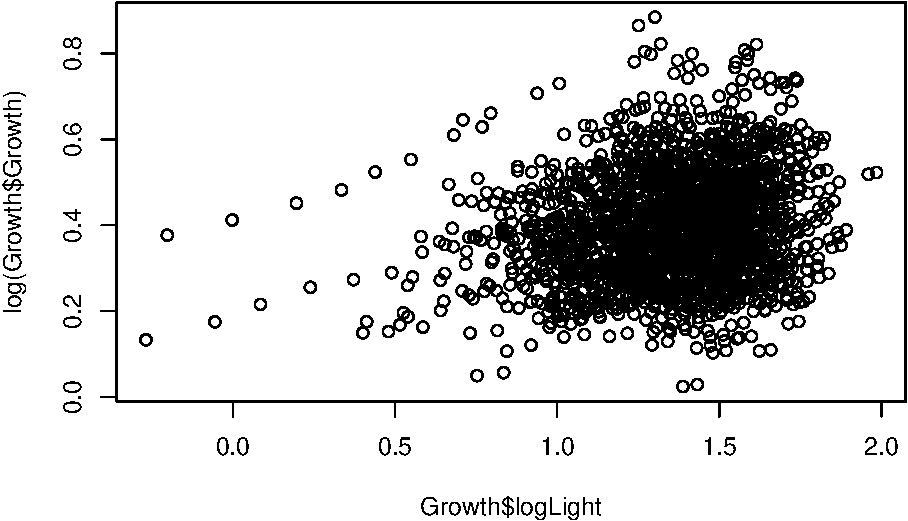
\includegraphics{theoretical_model_files/figure-latex/Growth plots-1.pdf}
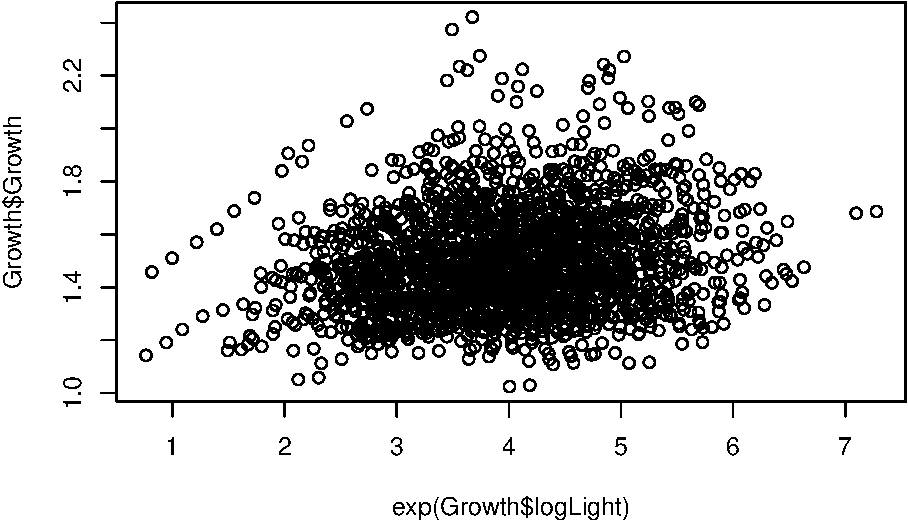
\includegraphics{theoretical_model_files/figure-latex/Growth plots-2.pdf}
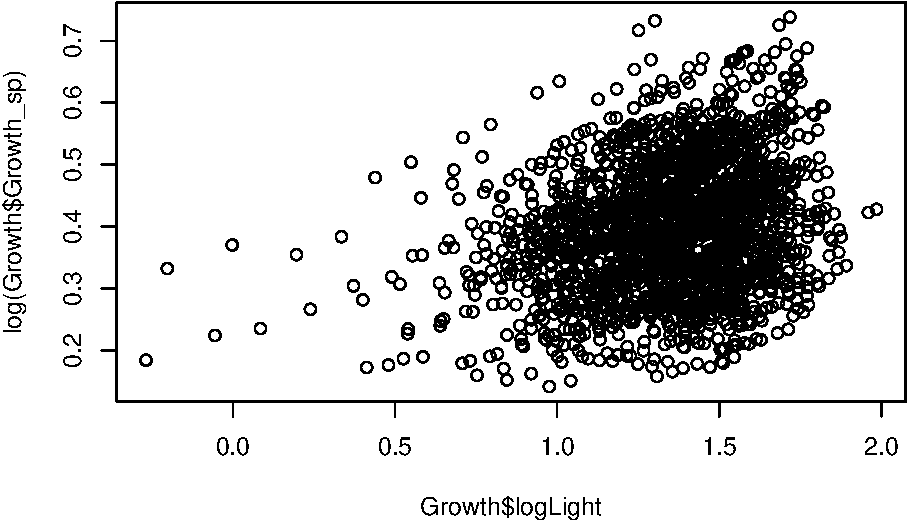
\includegraphics{theoretical_model_files/figure-latex/Growth plots-3.pdf}
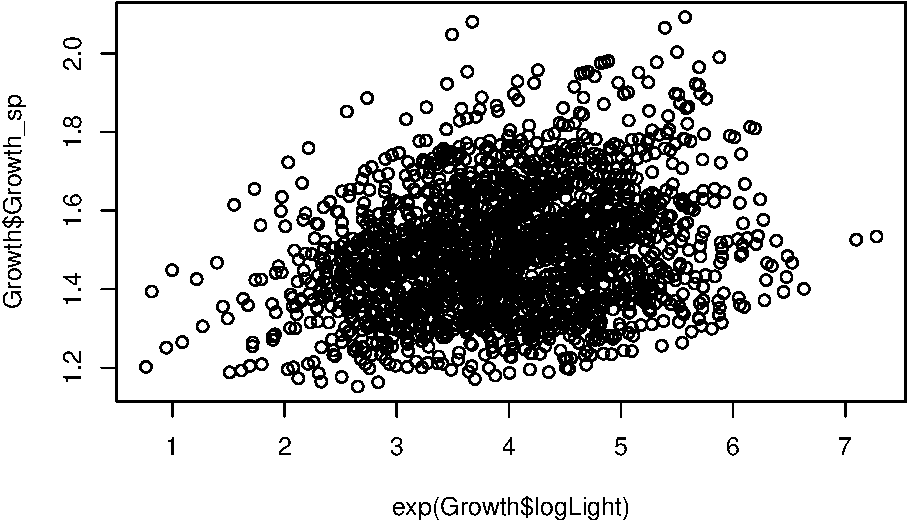
\includegraphics{theoretical_model_files/figure-latex/Growth plots-4.pdf}
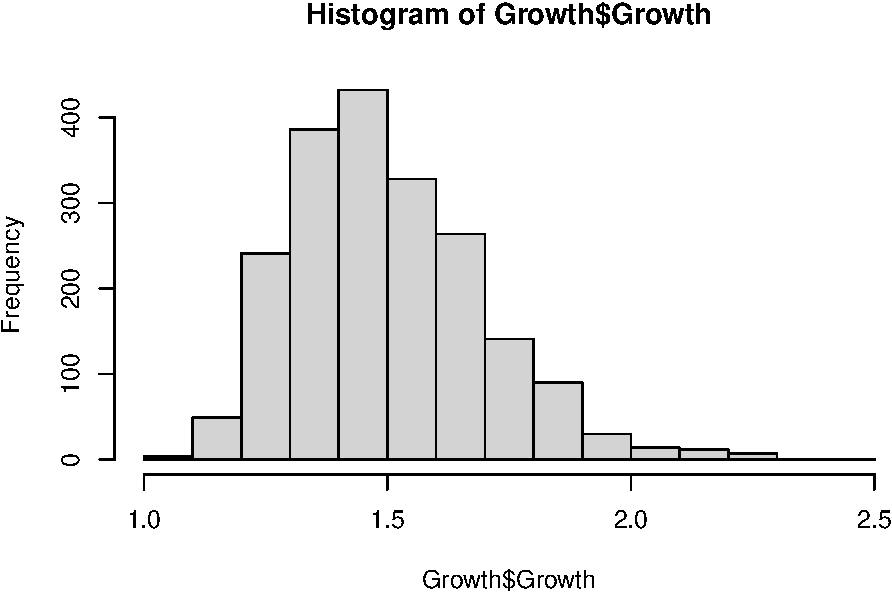
\includegraphics{theoretical_model_files/figure-latex/Growth plots-5.pdf}
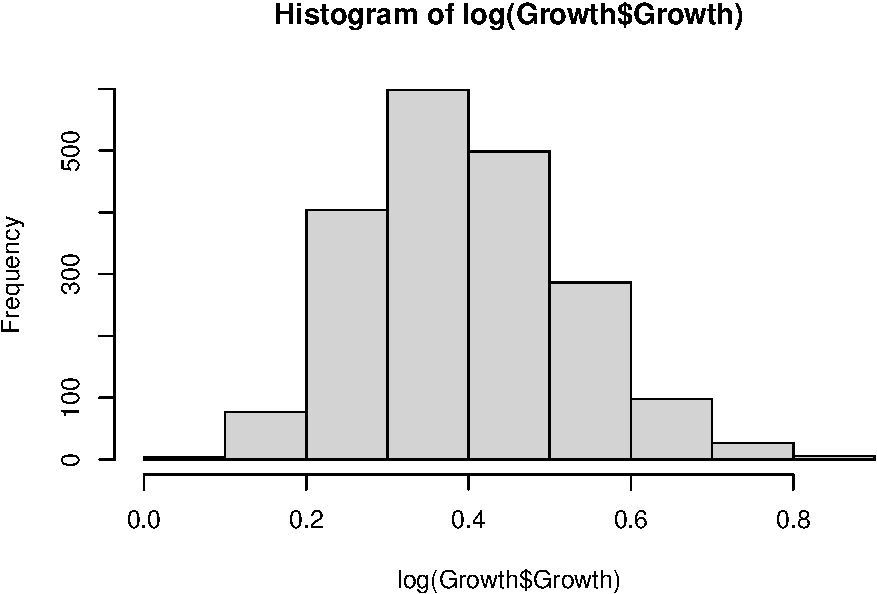
\includegraphics{theoretical_model_files/figure-latex/Growth plots-6.pdf}
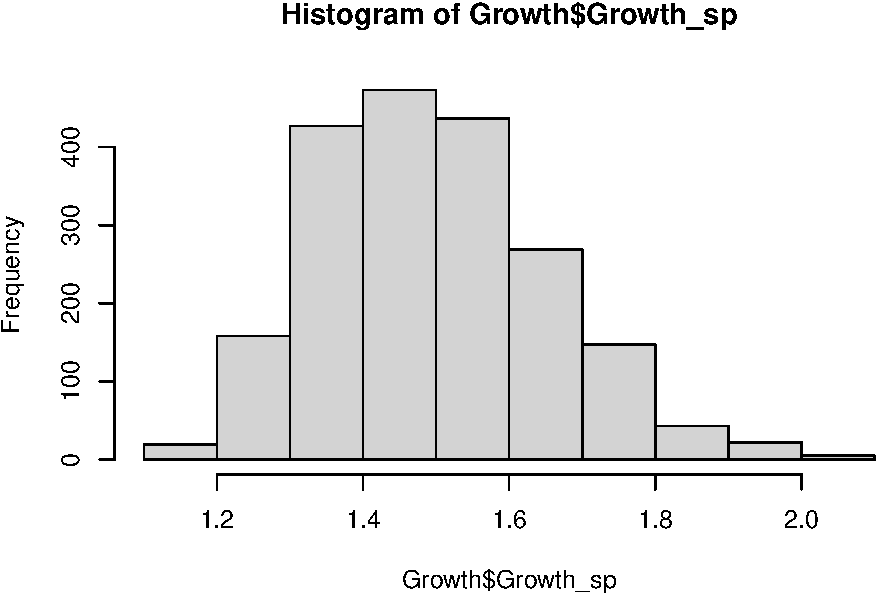
\includegraphics{theoretical_model_files/figure-latex/Growth plots-7.pdf}
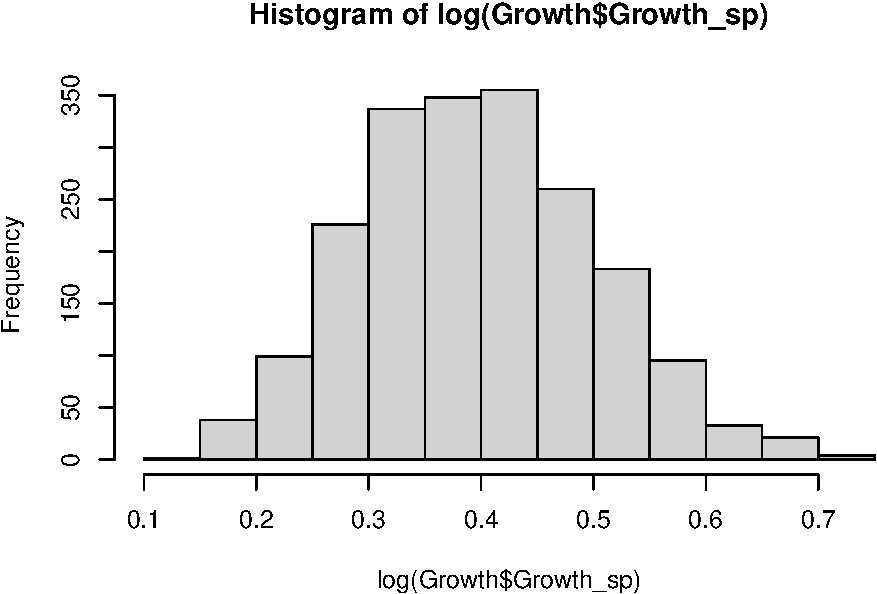
\includegraphics{theoretical_model_files/figure-latex/Growth plots-8.pdf}
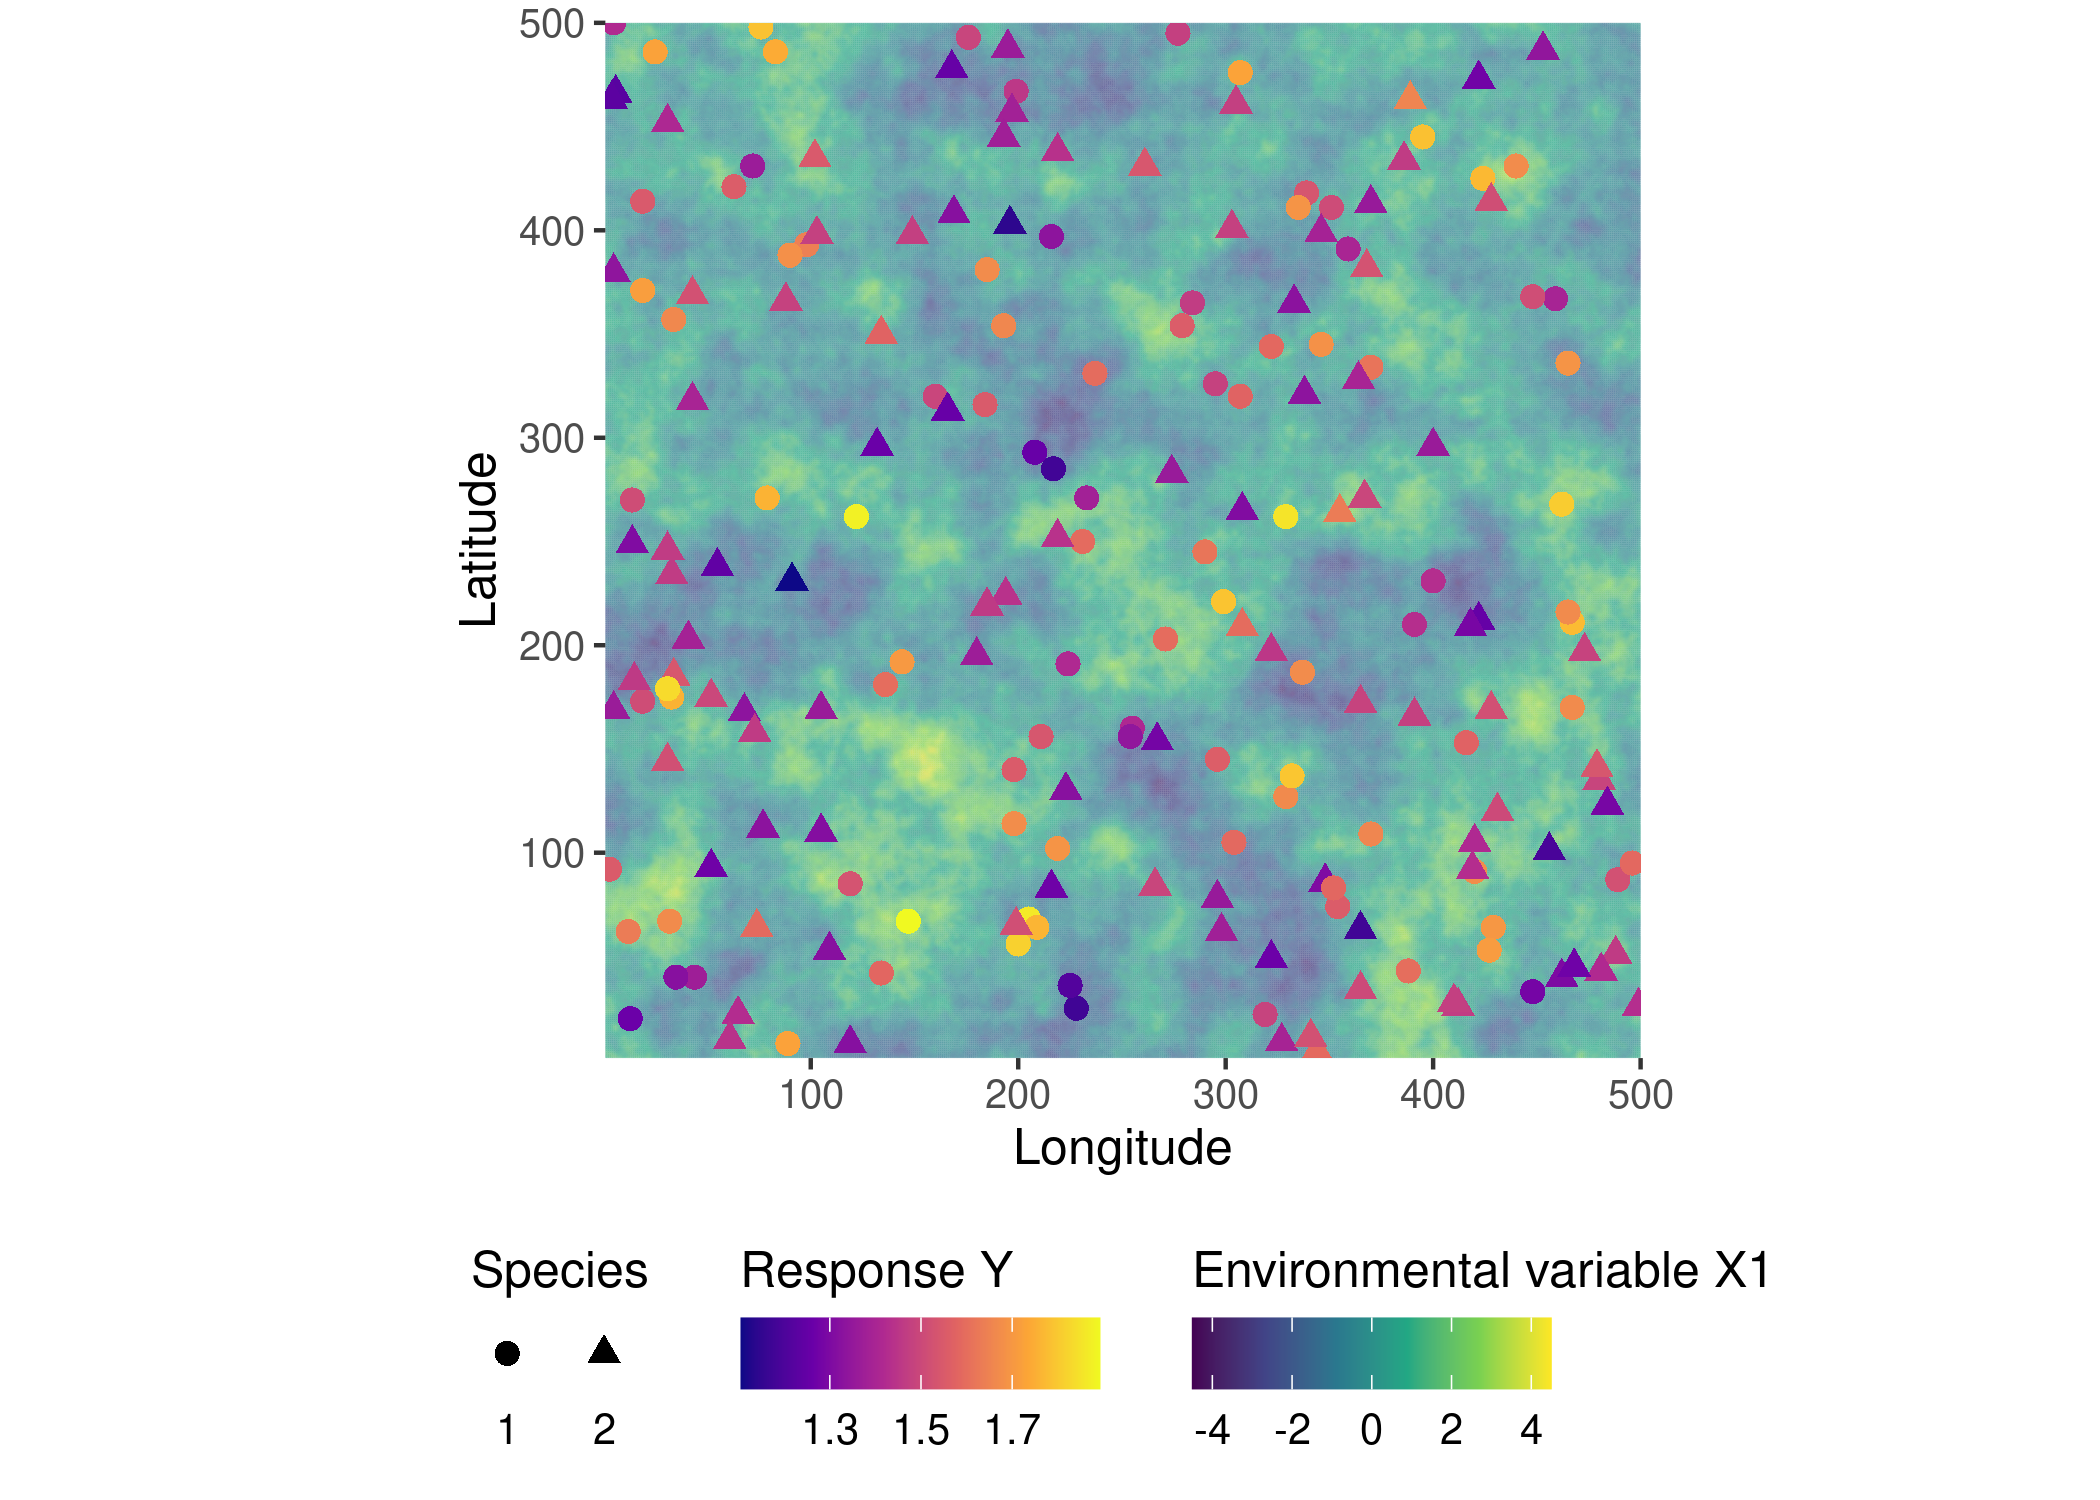
\includegraphics[width=29.17in]{/home/girard-tercieux/Code/coexIV/outputs/theoretical_model/figures/Map_growth}

On this figure, we can already see that microsite effects, which is the
effect of the local multidimensional environment on the observed
variable, can result in local reversals of the competitive hierarchy
between species, i.e.~the local outcome of competition can be opposite
to the mean hierarchy : at one point of the space-time, an individual of
Species 1 can overcome an individual of Species 2, whilst Species 1 is,
on average, the fittest of the two species. Doing this, microsite
effects foster the coexistence of Species 1 and Species 2.

\begin{Shaded}
\begin{Highlighting}[]
\NormalTok{Growth}\OperatorTok{$}\NormalTok{logGrowth <-}\StringTok{ }\KeywordTok{log}\NormalTok{(Growth}\OperatorTok{$}\NormalTok{Growth)}
\NormalTok{Growth}\OperatorTok{$}\NormalTok{logGrowth_sp <-}\StringTok{ }\KeywordTok{log}\NormalTok{(Growth}\OperatorTok{$}\NormalTok{Growth_sp)}
\end{Highlighting}
\end{Shaded}

\begin{Shaded}
\begin{Highlighting}[]
\CommentTok{# Statistical model with only one variable X}

\NormalTok{Data_brms_sp_}\DecValTok{1}\NormalTok{ <-}\StringTok{ }\KeywordTok{data.frame}\NormalTok{(}\DataTypeTok{Y =}\NormalTok{ Growth[}\KeywordTok{which}\NormalTok{(Growth}\OperatorTok{$}\NormalTok{Species }\OperatorTok{==}\StringTok{ }
\StringTok{    }\DecValTok{1}\NormalTok{), ]}\OperatorTok{$}\NormalTok{logGrowth_sp, }\DataTypeTok{X1 =}\NormalTok{ Growth[}\KeywordTok{which}\NormalTok{(Growth}\OperatorTok{$}\NormalTok{Species }\OperatorTok{==}\StringTok{ }\DecValTok{1}\NormalTok{), }
\NormalTok{    ]}\OperatorTok{$}\NormalTok{logLight, }\DataTypeTok{tree =}\NormalTok{ Growth[}\KeywordTok{which}\NormalTok{(Growth}\OperatorTok{$}\NormalTok{Species }\OperatorTok{==}\StringTok{ }\DecValTok{1}\NormalTok{), ]}\OperatorTok{$}\NormalTok{Ind)}
\CommentTok{# dplyr::mutate(Y=scale(Y), X1=scale(X1))}

\NormalTok{Data_brms_sp_}\DecValTok{2}\NormalTok{ <-}\StringTok{ }\KeywordTok{data.frame}\NormalTok{(}\DataTypeTok{Y =}\NormalTok{ Growth[}\KeywordTok{which}\NormalTok{(Growth}\OperatorTok{$}\NormalTok{Species }\OperatorTok{==}\StringTok{ }
\StringTok{    }\DecValTok{2}\NormalTok{), ]}\OperatorTok{$}\NormalTok{logGrowth_sp, }\DataTypeTok{X1 =}\NormalTok{ Growth[}\KeywordTok{which}\NormalTok{(Growth}\OperatorTok{$}\NormalTok{Species }\OperatorTok{==}\StringTok{ }\DecValTok{2}\NormalTok{), }
\NormalTok{    ]}\OperatorTok{$}\NormalTok{logLight, }\DataTypeTok{tree =}\NormalTok{ Growth[}\KeywordTok{which}\NormalTok{(Growth}\OperatorTok{$}\NormalTok{Species }\OperatorTok{==}\StringTok{ }\DecValTok{2}\NormalTok{), ]}\OperatorTok{$}\NormalTok{Ind)}
\CommentTok{# dplyr::mutate(Y=scale(Y), X1=scale(X1))}

\NormalTok{Data_brms_sp_}\DecValTok{1}\NormalTok{_IV <-}\StringTok{ }\KeywordTok{data.frame}\NormalTok{(}\DataTypeTok{Y =}\NormalTok{ Growth[}\KeywordTok{which}\NormalTok{(Growth}\OperatorTok{$}\NormalTok{Species }\OperatorTok{==}\StringTok{ }
\StringTok{    }\DecValTok{1}\NormalTok{), ]}\OperatorTok{$}\NormalTok{logGrowth, }\DataTypeTok{X1 =}\NormalTok{ Growth[}\KeywordTok{which}\NormalTok{(Growth}\OperatorTok{$}\NormalTok{Species }\OperatorTok{==}\StringTok{ }\DecValTok{1}\NormalTok{), }
\NormalTok{    ]}\OperatorTok{$}\NormalTok{logLight, }\DataTypeTok{tree =}\NormalTok{ Growth[}\KeywordTok{which}\NormalTok{(Growth}\OperatorTok{$}\NormalTok{Species }\OperatorTok{==}\StringTok{ }\DecValTok{1}\NormalTok{), ]}\OperatorTok{$}\NormalTok{Ind)}
\CommentTok{# dplyr::mutate(Y=scale(Y), X1=scale(X1))}

\NormalTok{Data_brms_sp_}\DecValTok{2}\NormalTok{_IV <-}\StringTok{ }\KeywordTok{data.frame}\NormalTok{(}\DataTypeTok{Y =}\NormalTok{ Growth[}\KeywordTok{which}\NormalTok{(Growth}\OperatorTok{$}\NormalTok{Species }\OperatorTok{==}\StringTok{ }
\StringTok{    }\DecValTok{2}\NormalTok{), ]}\OperatorTok{$}\NormalTok{logGrowth, }\DataTypeTok{X1 =}\NormalTok{ Growth[}\KeywordTok{which}\NormalTok{(Growth}\OperatorTok{$}\NormalTok{Species }\OperatorTok{==}\StringTok{ }\DecValTok{2}\NormalTok{), }
\NormalTok{    ]}\OperatorTok{$}\NormalTok{logLight, }\DataTypeTok{tree =}\NormalTok{ Growth[}\KeywordTok{which}\NormalTok{(Growth}\OperatorTok{$}\NormalTok{Species }\OperatorTok{==}\StringTok{ }\DecValTok{2}\NormalTok{), ]}\OperatorTok{$}\NormalTok{Ind)}
\CommentTok{# dplyr::mutate(Y=scale(Y), X1=scale(X1))}


\KeywordTok{options}\NormalTok{(}\DataTypeTok{m.cores =} \DecValTok{2}\NormalTok{)}

\CommentTok{### Priors}

\NormalTok{prior_brms <-}\StringTok{ }\KeywordTok{c}\NormalTok{(brms}\OperatorTok{::}\KeywordTok{prior}\NormalTok{(}\KeywordTok{normal}\NormalTok{(}\DecValTok{0}\NormalTok{, }\DecValTok{1}\NormalTok{), }\DataTypeTok{class =} \StringTok{"Intercept"}\NormalTok{), }
\NormalTok{    brms}\OperatorTok{::}\KeywordTok{prior}\NormalTok{(}\KeywordTok{normal}\NormalTok{(}\DecValTok{0}\NormalTok{, }\DecValTok{1}\NormalTok{), }\DataTypeTok{class =} \StringTok{"b"}\NormalTok{), brms}\OperatorTok{::}\KeywordTok{prior}\NormalTok{(}\KeywordTok{inv_gamma}\NormalTok{(}\DecValTok{10}\OperatorTok{^-}\DecValTok{3}\NormalTok{, }
        \DecValTok{10}\OperatorTok{^-}\DecValTok{3}\NormalTok{), }\DataTypeTok{class =} \StringTok{"sd"}\NormalTok{))}

\CommentTok{### Models}

\NormalTok{brms_mod_sp_}\DecValTok{1}\NormalTok{ <-}\StringTok{ }\NormalTok{brms}\OperatorTok{::}\KeywordTok{brm}\NormalTok{(}\DataTypeTok{formula =}\NormalTok{ Y }\OperatorTok{~}\StringTok{ }\DecValTok{1} \OperatorTok{+}\StringTok{ }\NormalTok{X1 }\OperatorTok{+}\StringTok{ }\NormalTok{(}\DecValTok{1} \OperatorTok{|}\StringTok{ }\NormalTok{tree), }
    \DataTypeTok{data =}\NormalTok{ Data_brms_sp_}\DecValTok{1}\NormalTok{, }\DataTypeTok{prior =}\NormalTok{ prior_brms, }\DataTypeTok{iter =} \FloatTok{1e+05}\NormalTok{, }
    \DataTypeTok{warmup =} \DecValTok{50000}\NormalTok{, }\DataTypeTok{thin =} \DecValTok{50}\NormalTok{, }\DataTypeTok{chains =} \DecValTok{2}\NormalTok{, }\DataTypeTok{cores =} \DecValTok{2}\NormalTok{)}

\KeywordTok{save}\NormalTok{(brms_mod_sp_}\DecValTok{1}\NormalTok{, }\DataTypeTok{file =}\NormalTok{ here}\OperatorTok{::}\KeywordTok{here}\NormalTok{(}\StringTok{"outputs"}\NormalTok{, }\StringTok{"theoretical_model"}\NormalTok{, }
    \StringTok{"brms_mod_sp_1.RData"}\NormalTok{))}

\NormalTok{brms_mod_sp_}\DecValTok{2}\NormalTok{ <-}\StringTok{ }\NormalTok{brms}\OperatorTok{::}\KeywordTok{brm}\NormalTok{(}\DataTypeTok{formula =}\NormalTok{ Y }\OperatorTok{~}\StringTok{ }\DecValTok{1} \OperatorTok{+}\StringTok{ }\NormalTok{X1 }\OperatorTok{+}\StringTok{ }\NormalTok{(}\DecValTok{1} \OperatorTok{|}\StringTok{ }\NormalTok{tree), }
    \DataTypeTok{data =}\NormalTok{ Data_brms_sp_}\DecValTok{2}\NormalTok{, }\DataTypeTok{prior =}\NormalTok{ prior_brms, }\DataTypeTok{iter =} \FloatTok{1e+05}\NormalTok{, }
    \DataTypeTok{warmup =} \DecValTok{50000}\NormalTok{, }\DataTypeTok{thin =} \DecValTok{50}\NormalTok{, }\DataTypeTok{chains =} \DecValTok{2}\NormalTok{, }\DataTypeTok{cores =} \DecValTok{2}\NormalTok{)}

\KeywordTok{save}\NormalTok{(brms_mod_sp_}\DecValTok{2}\NormalTok{, }\DataTypeTok{file =}\NormalTok{ here}\OperatorTok{::}\KeywordTok{here}\NormalTok{(}\StringTok{"outputs"}\NormalTok{, }\StringTok{"theoretical_model"}\NormalTok{, }
    \StringTok{"brms_mod_sp_2.RData"}\NormalTok{))}

\NormalTok{brms_mod_sp_}\DecValTok{1}\NormalTok{_IV <-}\StringTok{ }\NormalTok{brms}\OperatorTok{::}\KeywordTok{brm}\NormalTok{(}\DataTypeTok{formula =}\NormalTok{ Y }\OperatorTok{~}\StringTok{ }\DecValTok{1} \OperatorTok{+}\StringTok{ }\NormalTok{X1 }\OperatorTok{+}\StringTok{ }\NormalTok{(}\DecValTok{1} \OperatorTok{|}\StringTok{ }\NormalTok{tree), }
    \DataTypeTok{data =}\NormalTok{ Data_brms_sp_}\DecValTok{1}\NormalTok{_IV, }\DataTypeTok{prior =}\NormalTok{ prior_brms, }\DataTypeTok{iter =} \FloatTok{1e+05}\NormalTok{, }
    \DataTypeTok{warmup =} \DecValTok{50000}\NormalTok{, }\DataTypeTok{thin =} \DecValTok{50}\NormalTok{, }\DataTypeTok{chains =} \DecValTok{2}\NormalTok{, }\DataTypeTok{cores =} \DecValTok{2}\NormalTok{)}

\KeywordTok{save}\NormalTok{(brms_mod_sp_}\DecValTok{1}\NormalTok{_IV, }\DataTypeTok{file =}\NormalTok{ here}\OperatorTok{::}\KeywordTok{here}\NormalTok{(}\StringTok{"outputs"}\NormalTok{, }\StringTok{"theoretical_model"}\NormalTok{, }
    \StringTok{"brms_mod_sp_1_IV.RData"}\NormalTok{))}

\NormalTok{brms_mod_sp_}\DecValTok{2}\NormalTok{_IV <-}\StringTok{ }\NormalTok{brms}\OperatorTok{::}\KeywordTok{brm}\NormalTok{(}\DataTypeTok{formula =}\NormalTok{ Y }\OperatorTok{~}\StringTok{ }\DecValTok{1} \OperatorTok{+}\StringTok{ }\NormalTok{X1 }\OperatorTok{+}\StringTok{ }\NormalTok{(}\DecValTok{1} \OperatorTok{|}\StringTok{ }\NormalTok{tree), }
    \DataTypeTok{data =}\NormalTok{ Data_brms_sp_}\DecValTok{2}\NormalTok{_IV, }\DataTypeTok{prior =}\NormalTok{ prior_brms, }\DataTypeTok{iter =} \FloatTok{1e+05}\NormalTok{, }
    \DataTypeTok{warmup =} \DecValTok{50000}\NormalTok{, }\DataTypeTok{thin =} \DecValTok{50}\NormalTok{, }\DataTypeTok{chains =} \DecValTok{2}\NormalTok{, }\DataTypeTok{cores =} \DecValTok{2}\NormalTok{)}

\KeywordTok{save}\NormalTok{(brms_mod_sp_}\DecValTok{2}\NormalTok{_IV, }\DataTypeTok{file =}\NormalTok{ here}\OperatorTok{::}\KeywordTok{here}\NormalTok{(}\StringTok{"outputs"}\NormalTok{, }\StringTok{"theoretical_model"}\NormalTok{, }
    \StringTok{"brms_mod_sp_2_IV.RData"}\NormalTok{))}
\end{Highlighting}
\end{Shaded}

We visualise the convergence and the results of the models thanks to
trace and density plots and the summary of the models.

\begin{verbatim}
## Warning: Parts of the model have not converged (some Rhats are > 1.05). Be careful when
## analysing the results! We recommend running more iterations and/or setting stronger priors.
\end{verbatim}

\begin{table}[!h]
\centering
\begin{tabular}[t]{lllll}
\toprule
  & $\beta_0$ & $\beta_1$ & $V_b$ & $V$\\
\midrule
\addlinespace[0.3em]
\multicolumn{5}{l}{\textbf{Species 1}}\\
\cellcolor{gray!6}{\hspace{1em}Estimate} & \cellcolor{gray!6}{6.4e-02} & \cellcolor{gray!6}{2.9e-01} & \cellcolor{gray!6}{9.5e-02} & \cellcolor{gray!6}{1.9e-03}\\
\hspace{1em}Estimation error & 4.7e-03 & 2.4e-03 & 3e-03 & 6.1e-05\\
\addlinespace[0.3em]
\multicolumn{5}{l}{\textbf{Species 2}}\\
\cellcolor{gray!6}{\hspace{1em}Estimate} & \cellcolor{gray!6}{1.3e-01} & \cellcolor{gray!6}{1.5e-01} & \cellcolor{gray!6}{7.6e-02} & \cellcolor{gray!6}{5.2e-04}\\
\hspace{1em}Estimation error & 3.3e-03 & 6.3e-04 & 2.4e-03 & 1.7e-05\\
\bottomrule
\end{tabular}
\end{table}

We infer a high intraspecific variability even in the absence of genetic
intraspecific variability. Therefore, observed intraspecific variability
does not necessarily reveal intrinsic (mainly genetic) intraspecific
variability, but can also reveal hidden dimensions of the environment.

The mean and quantiles of the results of the models are used to
visualise the inferred link between \(Y\) and \(X1\). To do so, we
create a sequence of explanatory variable values and compute the
response variable with the parameters inferred with the models.

\begin{Shaded}
\begin{Highlighting}[]
\CommentTok{# Create a sequence of 100 values of X (which is light for}
\CommentTok{# instance)}
\NormalTok{npred <-}\StringTok{ }\DecValTok{100}
\NormalTok{logLight_seq <-}\StringTok{ }\KeywordTok{seq}\NormalTok{(}\KeywordTok{min}\NormalTok{(Growth}\OperatorTok{$}\NormalTok{logLight), }\KeywordTok{max}\NormalTok{(Growth}\OperatorTok{$}\NormalTok{logLight), }
    \DataTypeTok{length.out =}\NormalTok{ npred)}
\NormalTok{Sd_b_IV <-}\StringTok{ }\KeywordTok{mean}\NormalTok{(}\KeywordTok{c}\NormalTok{(MCMC_brms_sp_}\DecValTok{1}\NormalTok{_IV[[}\DecValTok{1}\NormalTok{]][, }\DecValTok{3}\NormalTok{], MCMC_brms_sp_}\DecValTok{1}\NormalTok{_IV[[}\DecValTok{2}\NormalTok{]][, }
    \DecValTok{3}\NormalTok{]))}
\NormalTok{Sd_b_sp <-}\StringTok{ }\KeywordTok{mean}\NormalTok{(}\KeywordTok{c}\NormalTok{(MCMC_brms_sp_}\DecValTok{1}\NormalTok{[[}\DecValTok{1}\NormalTok{]][, }\DecValTok{3}\NormalTok{], MCMC_brms_sp_}\DecValTok{1}\NormalTok{[[}\DecValTok{2}\NormalTok{]][, }
    \DecValTok{3}\NormalTok{]))}

\CommentTok{# Without genetic variation#}
\NormalTok{Param_}\DecValTok{1}\NormalTok{_sp <-}\StringTok{ }\KeywordTok{data.frame}\NormalTok{(}\DataTypeTok{b1.1 =} \KeywordTok{numeric}\NormalTok{(}\DecValTok{2000}\NormalTok{), }\DataTypeTok{b1.2 =} \KeywordTok{numeric}\NormalTok{(}\DecValTok{2000}\NormalTok{), }
    \DataTypeTok{ind =} \KeywordTok{numeric}\NormalTok{(}\DecValTok{2000}\NormalTok{))}
\NormalTok{Param_}\DecValTok{1}\NormalTok{_sp[, }\DecValTok{1}\NormalTok{] <-}\StringTok{ }\KeywordTok{c}\NormalTok{(MCMC_brms_sp_}\DecValTok{1}\NormalTok{[[}\DecValTok{1}\NormalTok{]][, }\DecValTok{1}\NormalTok{], MCMC_brms_sp_}\DecValTok{1}\NormalTok{[[}\DecValTok{2}\NormalTok{]][, }
    \DecValTok{1}\NormalTok{])}
\NormalTok{Param_}\DecValTok{1}\NormalTok{_sp[, }\DecValTok{2}\NormalTok{] <-}\StringTok{ }\KeywordTok{c}\NormalTok{(MCMC_brms_sp_}\DecValTok{1}\NormalTok{[[}\DecValTok{1}\NormalTok{]][, }\DecValTok{2}\NormalTok{], MCMC_brms_sp_}\DecValTok{1}\NormalTok{[[}\DecValTok{2}\NormalTok{]][, }
    \DecValTok{2}\NormalTok{])}
\NormalTok{Param_}\DecValTok{1}\NormalTok{_sp[, }\DecValTok{3}\NormalTok{] <-}\StringTok{ }\KeywordTok{rnorm}\NormalTok{(}\DecValTok{2000}\NormalTok{, }\DecValTok{0}\NormalTok{, Sd_b_sp)}
\NormalTok{Log_growth_pred_sp1_sp <-}\StringTok{ }\KeywordTok{matrix}\NormalTok{(}\DataTypeTok{nrow =} \DecValTok{2000}\NormalTok{, }\DataTypeTok{ncol =}\NormalTok{ npred)}
\ControlFlowTok{for}\NormalTok{ (n }\ControlFlowTok{in} \DecValTok{1}\OperatorTok{:}\NormalTok{npred) \{}
\NormalTok{    Log_growth_pred_sp1_sp[, n] <-}\StringTok{ }\NormalTok{Param_}\DecValTok{1}\NormalTok{_sp}\OperatorTok{$}\NormalTok{b1}\FloatTok{.1} \OperatorTok{+}\StringTok{ }\NormalTok{Param_}\DecValTok{1}\NormalTok{_sp}\OperatorTok{$}\NormalTok{b1}\FloatTok{.2} \OperatorTok{*}\StringTok{ }
\StringTok{        }\NormalTok{logLight_seq[n] }\OperatorTok{+}\StringTok{ }\NormalTok{Param_}\DecValTok{1}\NormalTok{_sp}\OperatorTok{$}\NormalTok{ind}
\NormalTok{\}}

\NormalTok{Param_}\DecValTok{2}\NormalTok{_sp <-}\StringTok{ }\KeywordTok{data.frame}\NormalTok{(}\DataTypeTok{b2.1 =} \KeywordTok{numeric}\NormalTok{(}\DecValTok{2000}\NormalTok{), }\DataTypeTok{b2.2 =} \KeywordTok{numeric}\NormalTok{(}\DecValTok{2000}\NormalTok{), }
    \DataTypeTok{ind =} \KeywordTok{numeric}\NormalTok{(}\DecValTok{2000}\NormalTok{))}
\NormalTok{Param_}\DecValTok{2}\NormalTok{_sp[, }\DecValTok{1}\NormalTok{] <-}\StringTok{ }\KeywordTok{c}\NormalTok{(MCMC_brms_sp_}\DecValTok{2}\NormalTok{[[}\DecValTok{1}\NormalTok{]][, }\DecValTok{1}\NormalTok{], MCMC_brms_sp_}\DecValTok{2}\NormalTok{[[}\DecValTok{2}\NormalTok{]][, }
    \DecValTok{1}\NormalTok{])}
\NormalTok{Param_}\DecValTok{2}\NormalTok{_sp[, }\DecValTok{2}\NormalTok{] <-}\StringTok{ }\KeywordTok{c}\NormalTok{(MCMC_brms_sp_}\DecValTok{2}\NormalTok{[[}\DecValTok{1}\NormalTok{]][, }\DecValTok{2}\NormalTok{], MCMC_brms_sp_}\DecValTok{2}\NormalTok{[[}\DecValTok{2}\NormalTok{]][, }
    \DecValTok{2}\NormalTok{])}
\NormalTok{Param_}\DecValTok{2}\NormalTok{_sp[, }\DecValTok{3}\NormalTok{] <-}\StringTok{ }\KeywordTok{rnorm}\NormalTok{(}\DecValTok{2000}\NormalTok{, }\DecValTok{0}\NormalTok{, Sd_b_sp)}
\NormalTok{Log_growth_pred_sp2_sp <-}\StringTok{ }\KeywordTok{matrix}\NormalTok{(}\DataTypeTok{nrow =} \DecValTok{2000}\NormalTok{, }\DataTypeTok{ncol =}\NormalTok{ npred)}
\ControlFlowTok{for}\NormalTok{ (n }\ControlFlowTok{in} \DecValTok{1}\OperatorTok{:}\NormalTok{npred) \{}
\NormalTok{    Log_growth_pred_sp2_sp[, n] <-}\StringTok{ }\NormalTok{Param_}\DecValTok{2}\NormalTok{_sp}\OperatorTok{$}\NormalTok{b2}\FloatTok{.1} \OperatorTok{+}\StringTok{ }\NormalTok{Param_}\DecValTok{2}\NormalTok{_sp}\OperatorTok{$}\NormalTok{b2}\FloatTok{.2} \OperatorTok{*}\StringTok{ }
\StringTok{        }\NormalTok{logLight_seq[n] }\OperatorTok{+}\StringTok{ }\NormalTok{Param_}\DecValTok{2}\NormalTok{_sp}\OperatorTok{$}\NormalTok{ind}
\NormalTok{\}}

\NormalTok{Mean_}\DecValTok{1}\NormalTok{_sp <-}\StringTok{ }\KeywordTok{apply}\NormalTok{(Log_growth_pred_sp1_sp, }\DecValTok{2}\NormalTok{, mean)}
\NormalTok{Quant_}\DecValTok{1}\NormalTok{_sp <-}\StringTok{ }\KeywordTok{apply}\NormalTok{(Log_growth_pred_sp1_sp, }\DecValTok{2}\NormalTok{, quantile, }\KeywordTok{c}\NormalTok{(}\FloatTok{0.025}\NormalTok{, }
    \FloatTok{0.975}\NormalTok{))}
\NormalTok{Mean_}\DecValTok{2}\NormalTok{_sp <-}\StringTok{ }\KeywordTok{apply}\NormalTok{(Log_growth_pred_sp2_sp, }\DecValTok{2}\NormalTok{, mean)}
\NormalTok{Quant_}\DecValTok{2}\NormalTok{_sp <-}\StringTok{ }\KeywordTok{apply}\NormalTok{(Log_growth_pred_sp2_sp, }\DecValTok{2}\NormalTok{, quantile, }\KeywordTok{c}\NormalTok{(}\FloatTok{0.025}\NormalTok{, }
    \FloatTok{0.975}\NormalTok{))}

\NormalTok{Marg_}\DecValTok{1}\NormalTok{_sp <-}\StringTok{ }\KeywordTok{data.frame}\NormalTok{(logLight_seq, }\DataTypeTok{Mean_sp =}\NormalTok{ Mean_}\DecValTok{1}\NormalTok{_sp, }\DataTypeTok{Q025_sp =}\NormalTok{ Quant_}\DecValTok{1}\NormalTok{_sp[}\DecValTok{1}\NormalTok{, }
\NormalTok{    ], }\DataTypeTok{Q975_sp =}\NormalTok{ Quant_}\DecValTok{1}\NormalTok{_sp[}\DecValTok{2}\NormalTok{, ])}
\NormalTok{Marg_}\DecValTok{2}\NormalTok{_sp <-}\StringTok{ }\KeywordTok{data.frame}\NormalTok{(logLight_seq, }\DataTypeTok{Mean_sp =}\NormalTok{ Mean_}\DecValTok{2}\NormalTok{_sp, }\DataTypeTok{Q025_sp =}\NormalTok{ Quant_}\DecValTok{2}\NormalTok{_sp[}\DecValTok{1}\NormalTok{, }
\NormalTok{    ], }\DataTypeTok{Q975_sp =}\NormalTok{ Quant_}\DecValTok{2}\NormalTok{_sp[}\DecValTok{2}\NormalTok{, ])}

\NormalTok{Marg_sp <-}\StringTok{ }\KeywordTok{rbind}\NormalTok{(Marg_}\DecValTok{1}\NormalTok{_sp, Marg_}\DecValTok{2}\NormalTok{_sp)}
\KeywordTok{names}\NormalTok{(Marg_sp) <-}\StringTok{ }\KeywordTok{c}\NormalTok{(}\StringTok{"logLight"}\NormalTok{, }\StringTok{"logGrowth_sp"}\NormalTok{, }\StringTok{"logQ025_sp"}\NormalTok{, }
    \StringTok{"logQ975_sp"}\NormalTok{)}
\NormalTok{Marg_sp}\OperatorTok{$}\NormalTok{Species <-}\StringTok{ }\KeywordTok{rep}\NormalTok{(}\KeywordTok{c}\NormalTok{(}\DecValTok{1}\NormalTok{, }\DecValTok{2}\NormalTok{), }\DataTypeTok{each =}\NormalTok{ npred)}
\NormalTok{Marg_sp}\OperatorTok{$}\NormalTok{Species <-}\StringTok{ }\KeywordTok{as.factor}\NormalTok{(Marg_sp}\OperatorTok{$}\NormalTok{Species)}

\CommentTok{# Use exponential to draw a logarithmical curve}
\NormalTok{Marg_sp}\OperatorTok{$}\NormalTok{Light <-}\StringTok{ }\KeywordTok{exp}\NormalTok{(Marg_sp}\OperatorTok{$}\NormalTok{logLight)}
\NormalTok{Marg_sp}\OperatorTok{$}\NormalTok{Growth_sp <-}\StringTok{ }\KeywordTok{exp}\NormalTok{(Marg_sp}\OperatorTok{$}\NormalTok{logGrowth_sp)}
\NormalTok{Marg_sp}\OperatorTok{$}\NormalTok{Q025_sp <-}\StringTok{ }\KeywordTok{exp}\NormalTok{(Marg_sp}\OperatorTok{$}\NormalTok{logQ025_sp)}
\NormalTok{Marg_sp}\OperatorTok{$}\NormalTok{Q975_sp <-}\StringTok{ }\KeywordTok{exp}\NormalTok{(Marg_sp}\OperatorTok{$}\NormalTok{logQ975_sp)}

\NormalTok{Growth}\OperatorTok{$}\NormalTok{Light <-}\StringTok{ }\KeywordTok{exp}\NormalTok{(Growth}\OperatorTok{$}\NormalTok{logLight)}

\NormalTok{B <-}\StringTok{ }\NormalTok{ggplot2}\OperatorTok{::}\KeywordTok{ggplot}\NormalTok{(}\DataTypeTok{data =}\NormalTok{ Growth[}\KeywordTok{which}\NormalTok{(Growth}\OperatorTok{$}\NormalTok{Time }\OperatorTok{==}\StringTok{ }\DecValTok{1}\NormalTok{), ], }
\NormalTok{    ggplot2}\OperatorTok{::}\KeywordTok{aes}\NormalTok{(Light, Growth_sp)) }\OperatorTok{+}\StringTok{ }\NormalTok{ggplot2}\OperatorTok{::}\KeywordTok{geom_point}\NormalTok{(ggplot2}\OperatorTok{::}\KeywordTok{aes}\NormalTok{(}\DataTypeTok{colour =}\NormalTok{ Species)) }\OperatorTok{+}\StringTok{ }
\StringTok{    }\NormalTok{ggplot2}\OperatorTok{::}\KeywordTok{geom_line}\NormalTok{(}\DataTypeTok{data =}\NormalTok{ Marg_sp, }\DataTypeTok{size =} \DecValTok{1}\NormalTok{, ggplot2}\OperatorTok{::}\KeywordTok{aes}\NormalTok{(}\DataTypeTok{colour =}\NormalTok{ Species)) }\OperatorTok{+}\StringTok{ }
\StringTok{    }\NormalTok{ggplot2}\OperatorTok{::}\KeywordTok{geom_ribbon}\NormalTok{(}\DataTypeTok{data =}\NormalTok{ Marg_sp, }\DataTypeTok{alpha =} \FloatTok{0.2}\NormalTok{, ggplot2}\OperatorTok{::}\KeywordTok{aes}\NormalTok{(Light, }
        \DataTypeTok{ymin =}\NormalTok{ Q025_sp, }\DataTypeTok{ymax =}\NormalTok{ Q975_sp, }\DataTypeTok{colour =}\NormalTok{ Species, }\DataTypeTok{fill =}\NormalTok{ Species)) }\OperatorTok{+}\StringTok{ }
\StringTok{    }\NormalTok{ggplot2}\OperatorTok{::}\KeywordTok{coord_fixed}\NormalTok{(}\DataTypeTok{ratio =} \DecValTok{3}\NormalTok{) }\OperatorTok{+}\StringTok{ }\NormalTok{ggplot2}\OperatorTok{::}\KeywordTok{xlab}\NormalTok{(}\StringTok{"Observed environmnental variable (X1, e.g. light)"}\NormalTok{) }\OperatorTok{+}\StringTok{ }
\StringTok{    }\NormalTok{ggplot2}\OperatorTok{::}\KeywordTok{ylab}\NormalTok{(}\StringTok{"Response variables (Y, e.g. growth)"}\NormalTok{) }\OperatorTok{+}\StringTok{ }\NormalTok{ggplot2}\OperatorTok{::}\KeywordTok{guides}\NormalTok{(}\DataTypeTok{fill =}\NormalTok{ ggplot2}\OperatorTok{::}\KeywordTok{guide_legend}\NormalTok{(}\DataTypeTok{title.position =} \StringTok{"top"}\NormalTok{, }
    \DataTypeTok{label.position =} \StringTok{"bottom"}\NormalTok{)) }\OperatorTok{+}\StringTok{ }\NormalTok{ggplot2}\OperatorTok{::}\KeywordTok{theme}\NormalTok{(}\DataTypeTok{legend.position =} \StringTok{"bottom"}\NormalTok{, }
    \DataTypeTok{legend.title =}\NormalTok{ ggplot2}\OperatorTok{::}\KeywordTok{element_text}\NormalTok{(}\DataTypeTok{size =} \DecValTok{12}\NormalTok{), }\DataTypeTok{legend.text =}\NormalTok{ ggplot2}\OperatorTok{::}\KeywordTok{element_text}\NormalTok{(}\DataTypeTok{size =} \DecValTok{10}\NormalTok{), }
    \DataTypeTok{text =}\NormalTok{ ggplot2}\OperatorTok{::}\KeywordTok{element_text}\NormalTok{(}\DataTypeTok{size =} \DecValTok{12}\NormalTok{))}

\NormalTok{ggplot2}\OperatorTok{::}\KeywordTok{ggsave}\NormalTok{(}\DataTypeTok{filename =} \StringTok{"Partial_knowledge_model.png"}\NormalTok{, }\DataTypeTok{plot =}\NormalTok{ B, }
    \DataTypeTok{path =}\NormalTok{ here}\OperatorTok{::}\KeywordTok{here}\NormalTok{(}\StringTok{"outputs"}\NormalTok{, }\StringTok{"theoretical_model"}\NormalTok{, }\StringTok{"figures"}\NormalTok{), }
    \DataTypeTok{device =} \StringTok{"png"}\NormalTok{, }\DataTypeTok{width =} \DecValTok{7}\NormalTok{, }\DataTypeTok{height =} \DecValTok{5}\NormalTok{)}
\NormalTok{knitr}\OperatorTok{::}\KeywordTok{include_graphics}\NormalTok{(here}\OperatorTok{::}\KeywordTok{here}\NormalTok{(}\StringTok{"outputs"}\NormalTok{, }\StringTok{"theoretical_model"}\NormalTok{, }
    \StringTok{"figures"}\NormalTok{, }\StringTok{"Partial_knowledge_model.png"}\NormalTok{))}
\end{Highlighting}
\end{Shaded}

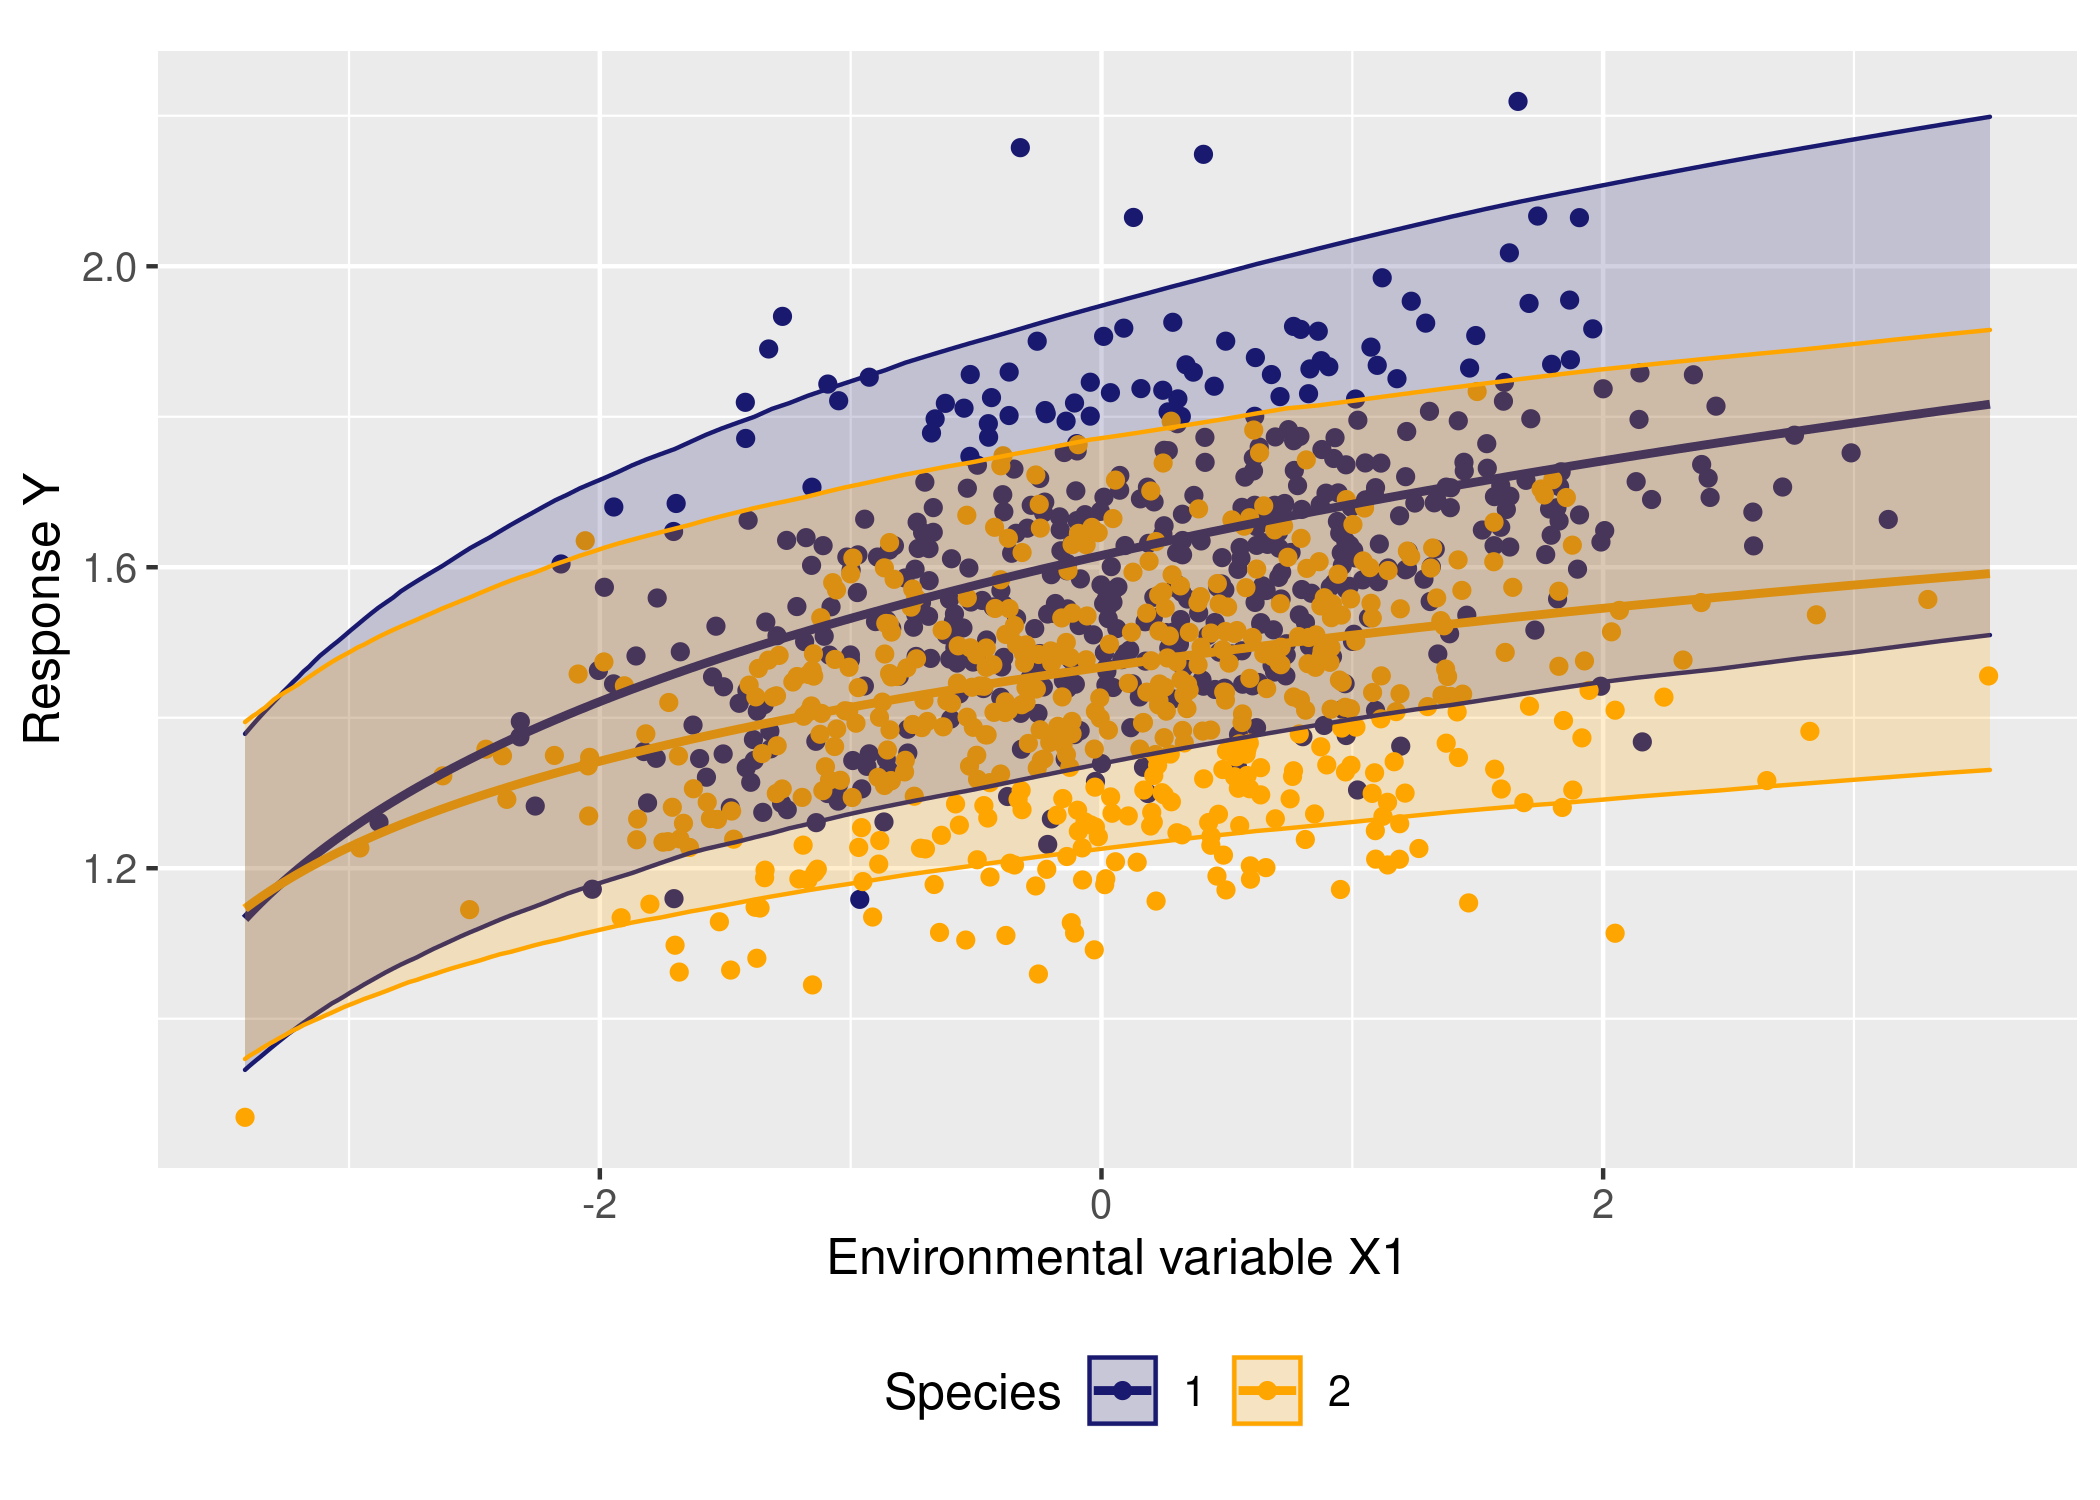
\includegraphics[width=29.17in]{/home/girard-tercieux/Code/coexIV/outputs/theoretical_model/figures/Partial_knowledge_model}

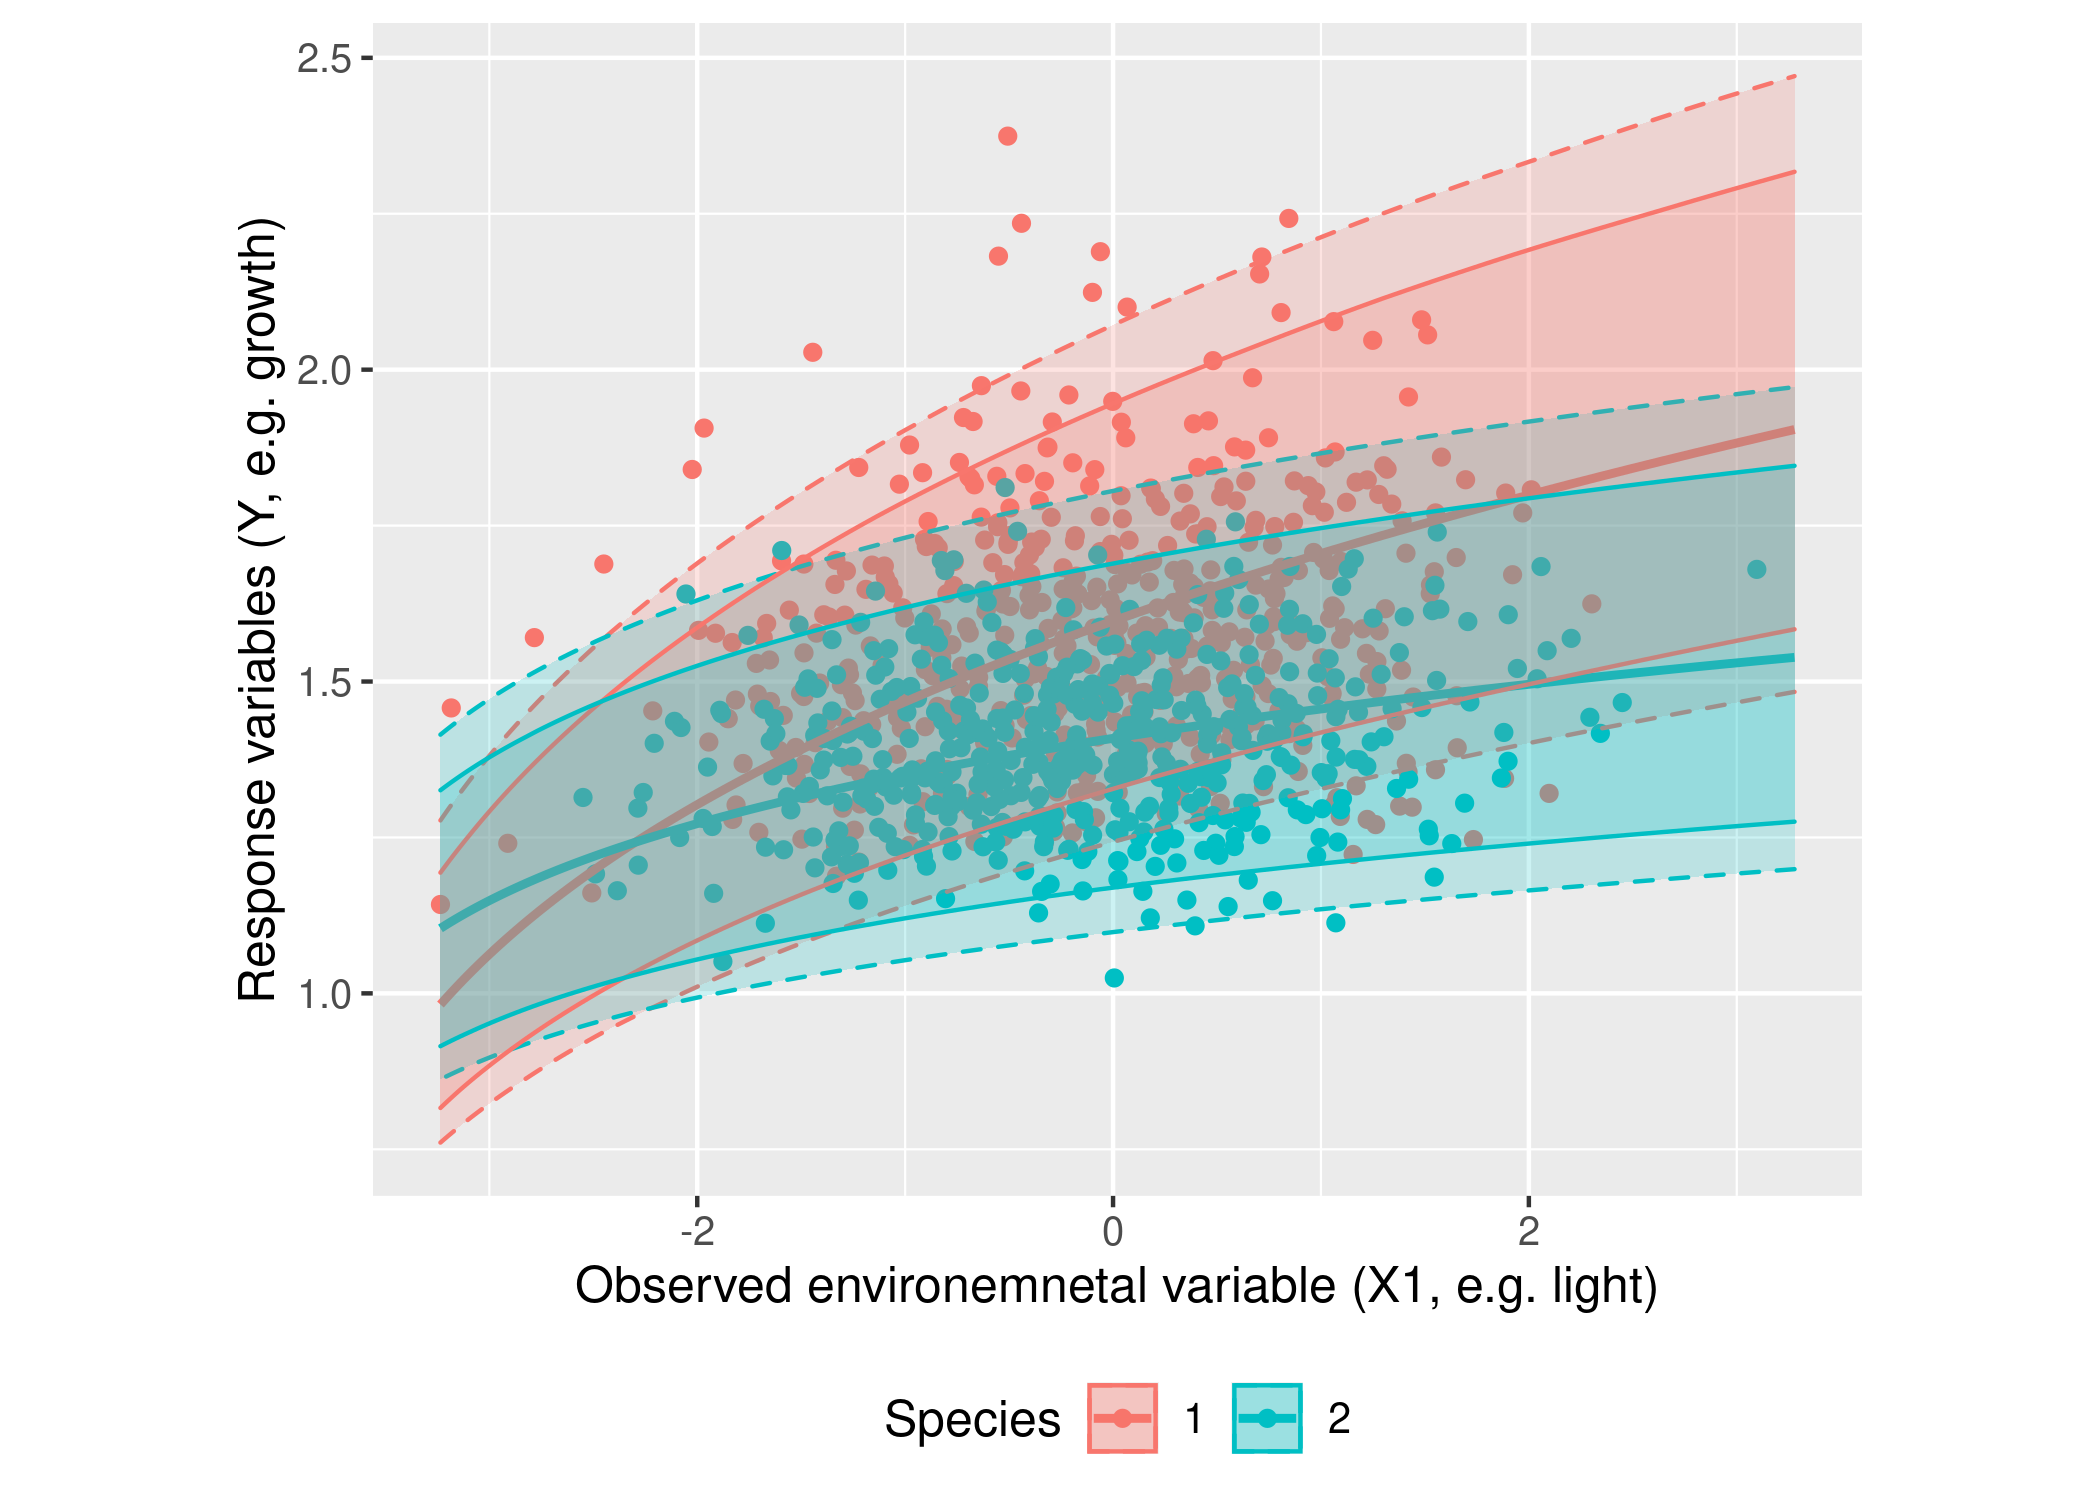
\includegraphics[width=29.17in]{/home/girard-tercieux/Code/coexIV/outputs/theoretical_model/figures/Partial_knowledge_model_genetic_var}

In these figures, the solid and bold lines represent the mean growth
rate of Species 1 (red) and Species 2 (blue) as computed with the
parameters retrieved from the model with or without genetic variability
respectively. The plain lines represent the 95\% interval of the
posteriors from the model without genetic variability and the dotted
lines show the 95\% confidence interval of the posteriors from the model
with genetic variability.

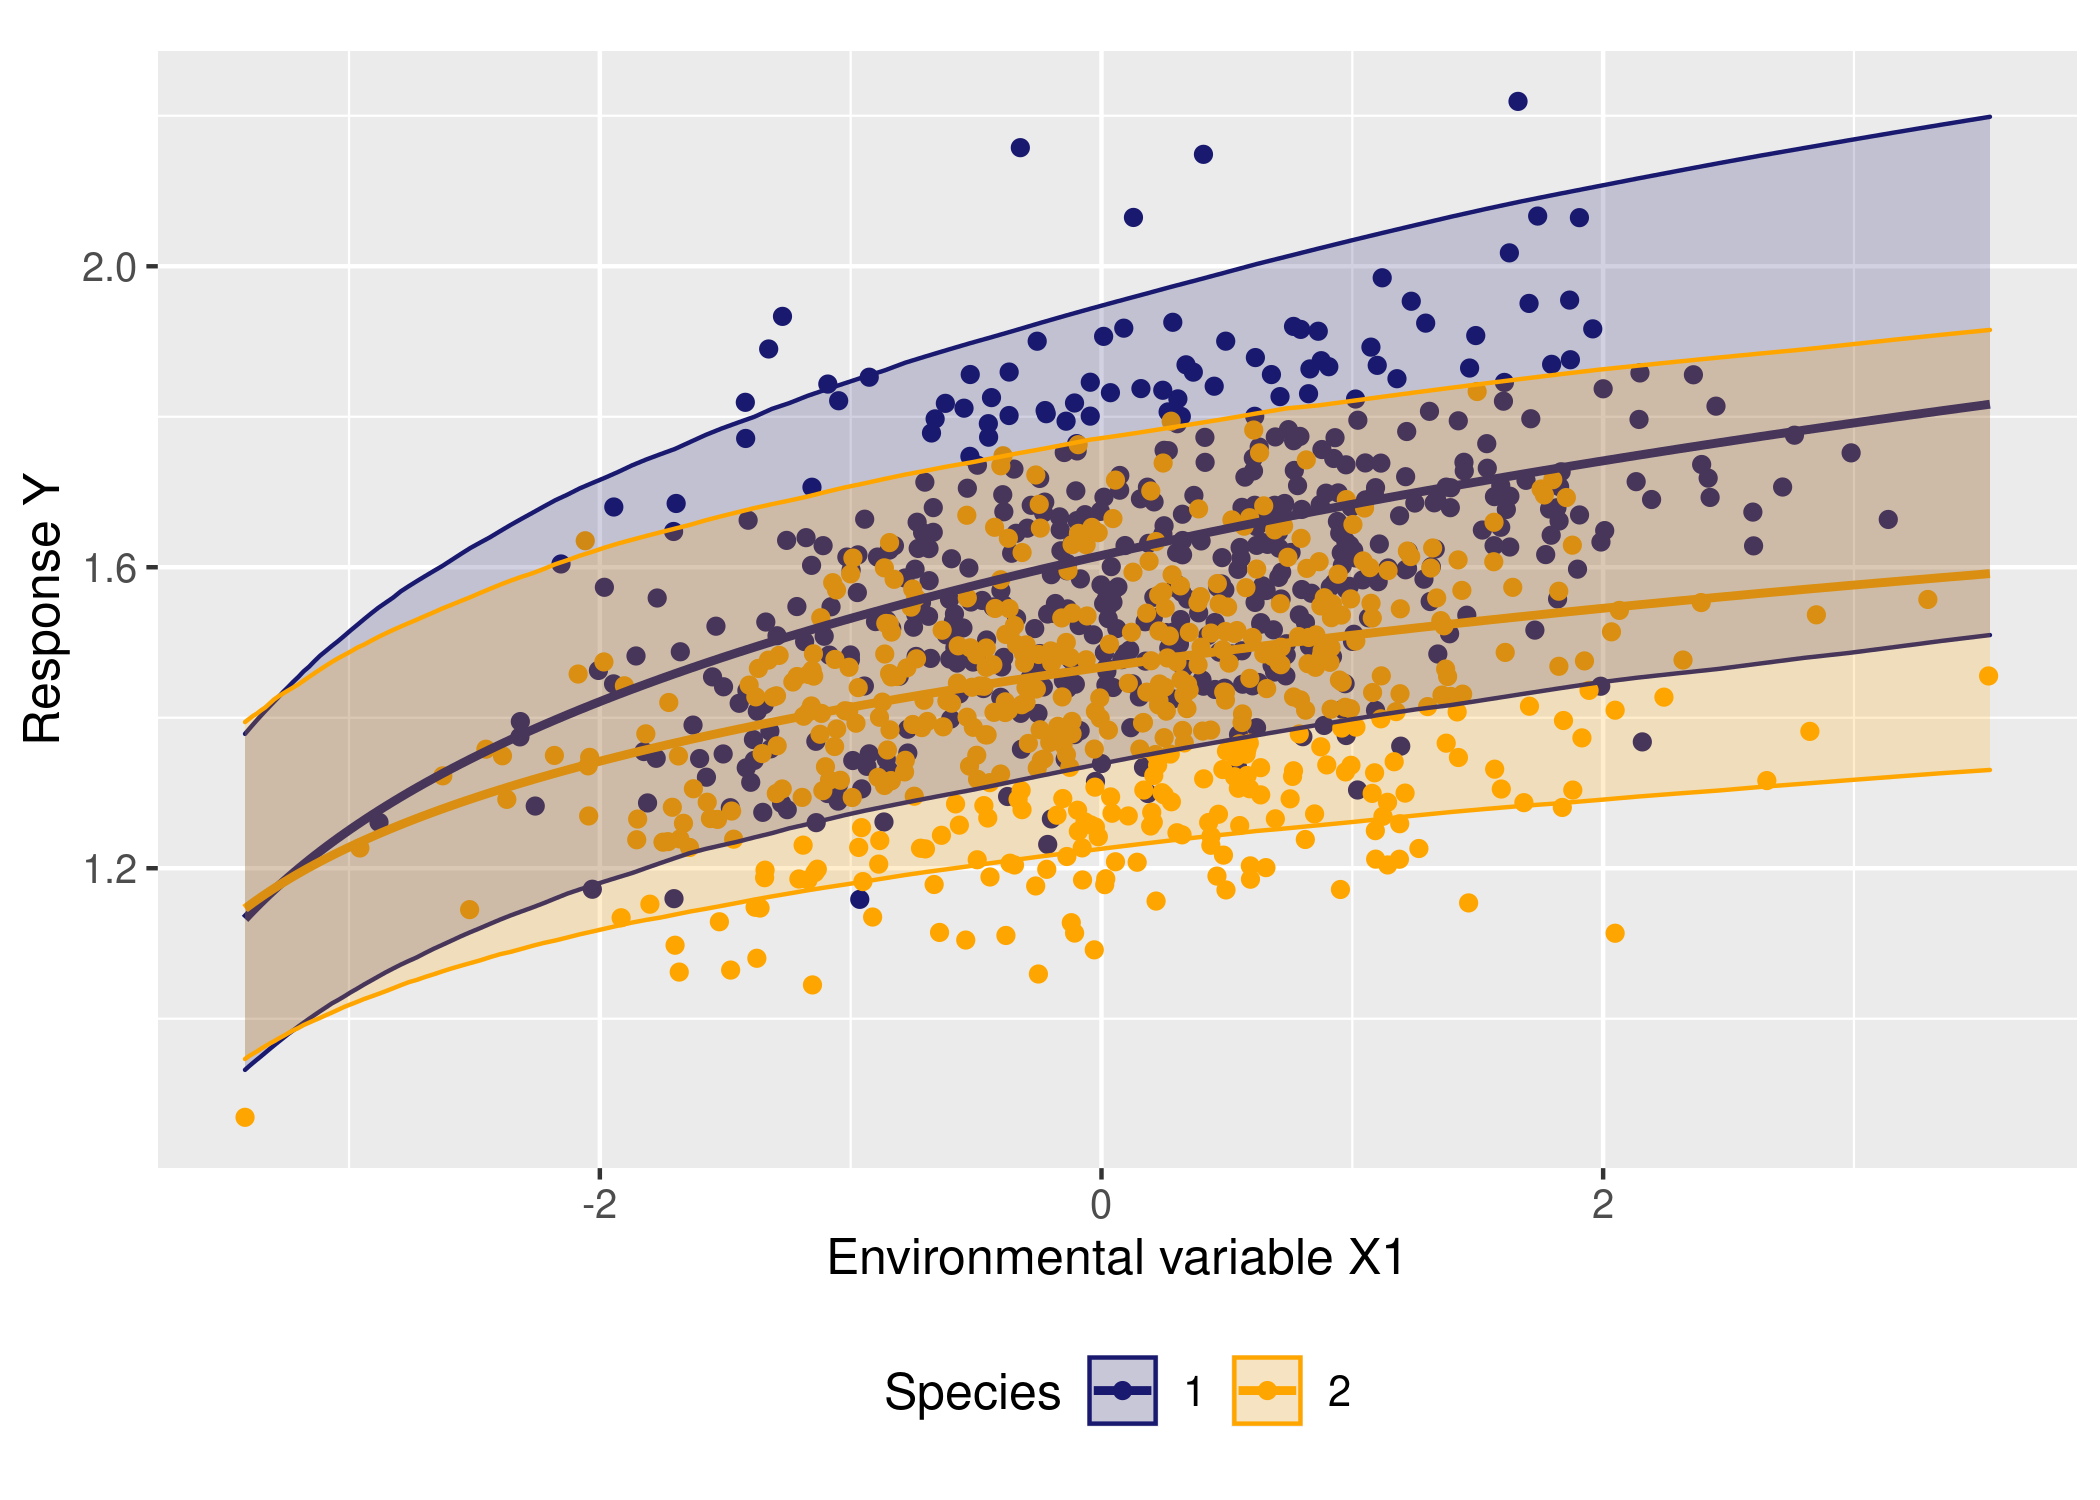
\includegraphics[width=0.5\linewidth]{/home/girard-tercieux/Code/coexIV/outputs/theoretical_model/figures/Partial_knowledge_model}
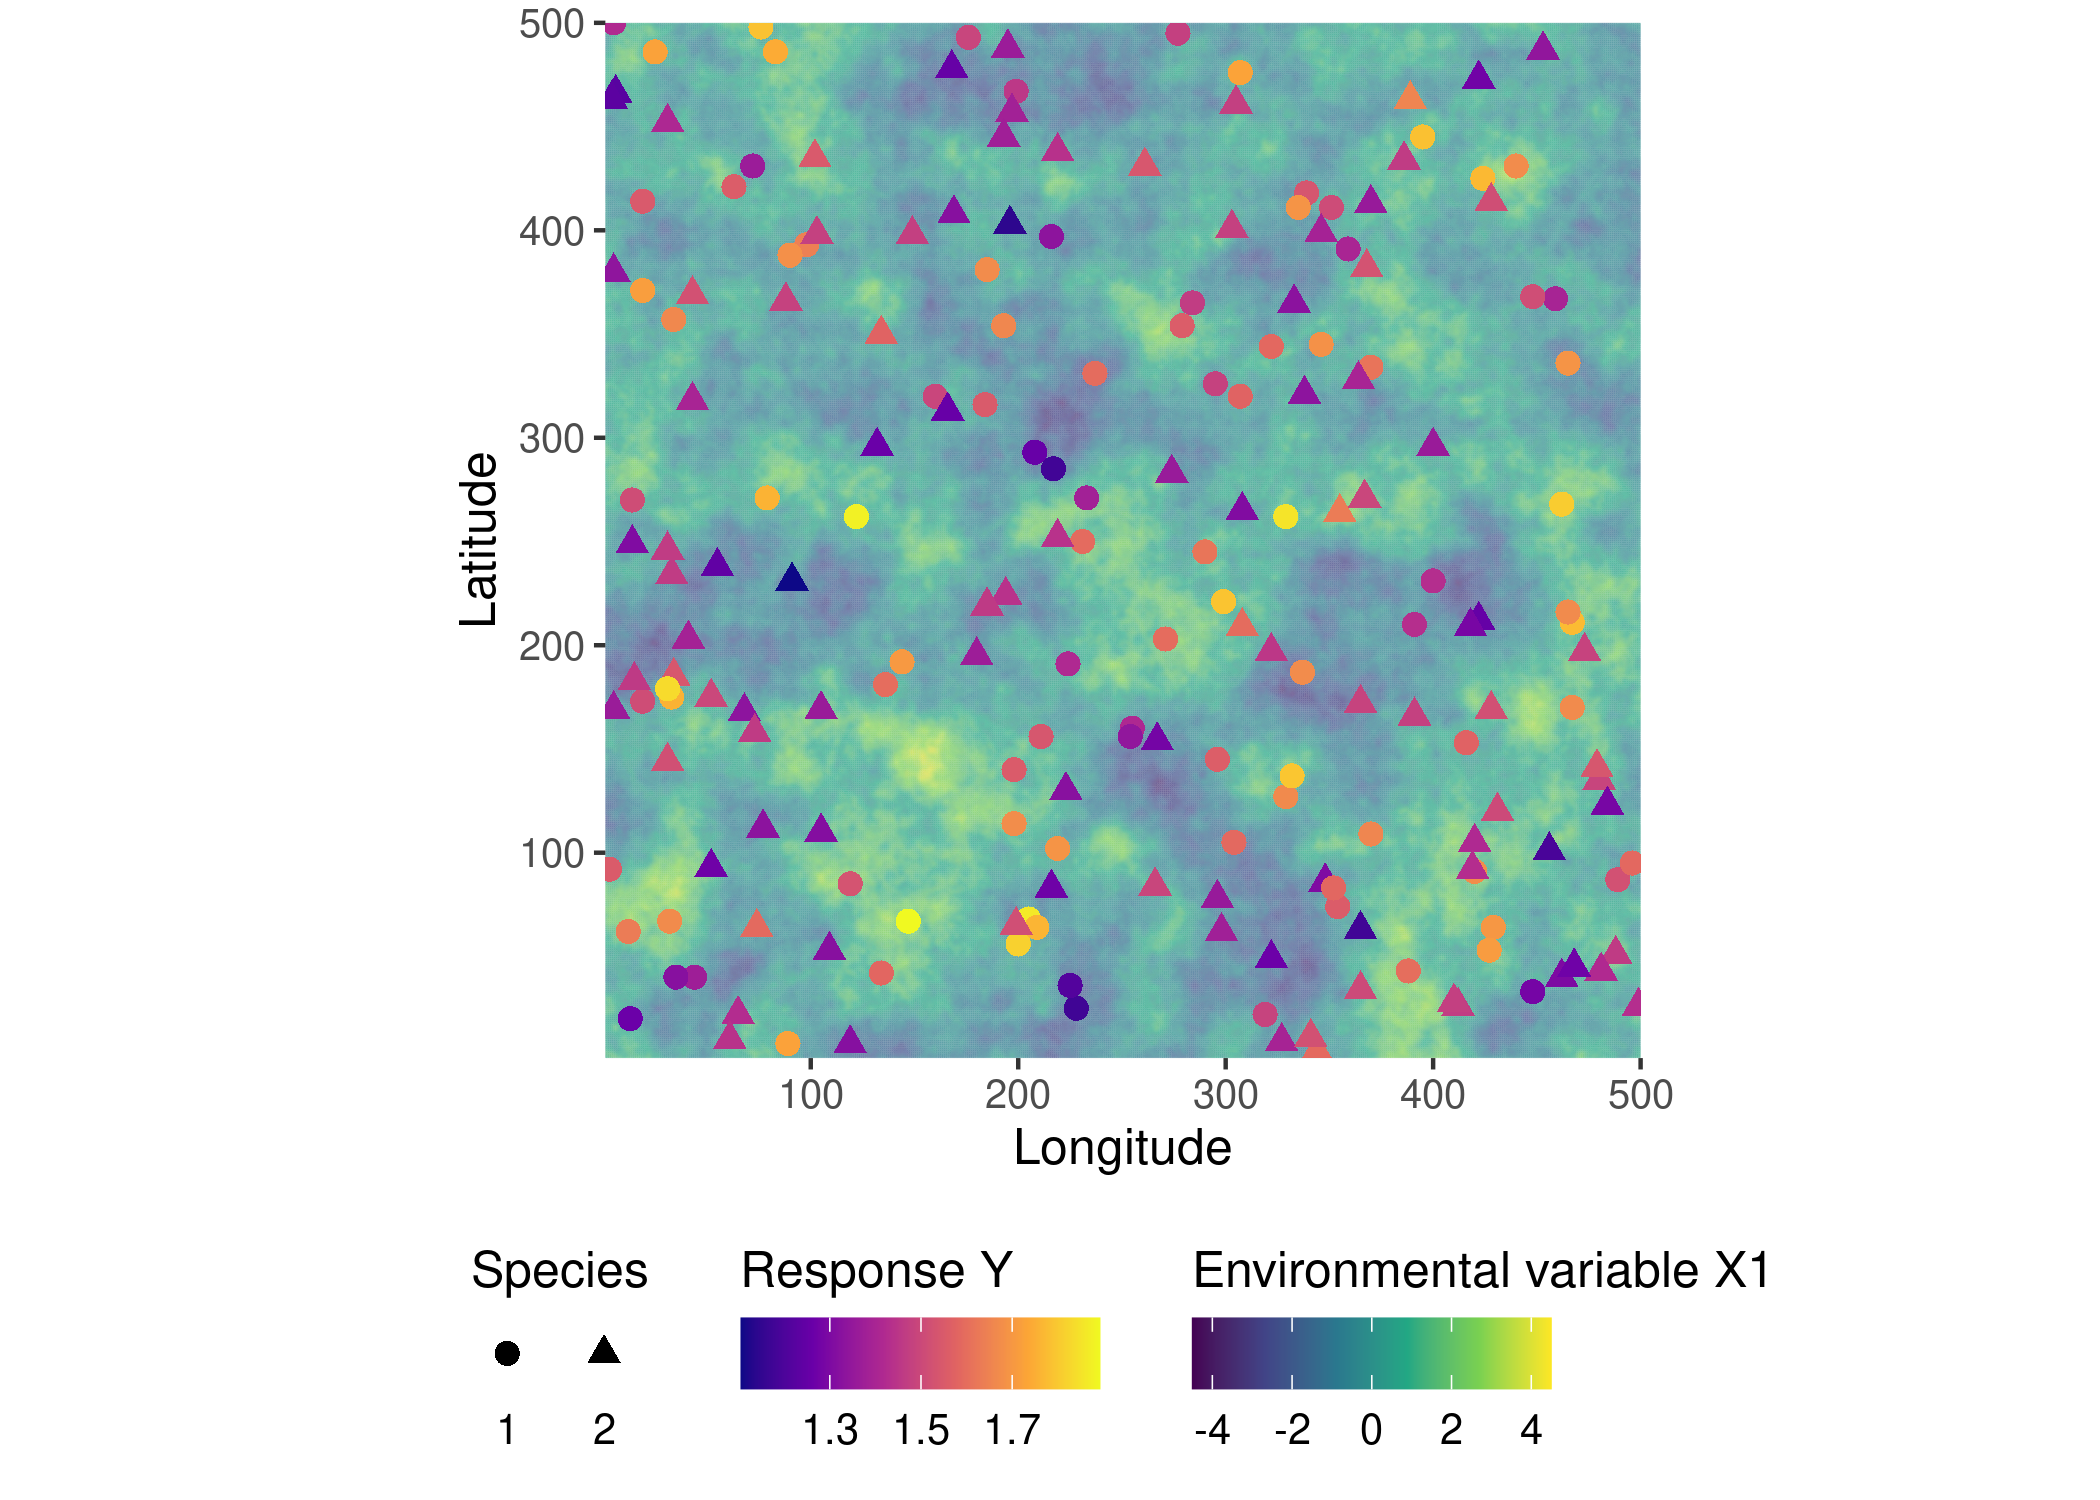
\includegraphics[width=0.5\linewidth]{/home/girard-tercieux/Code/coexIV/outputs/theoretical_model/figures/Map_growth}

In the model without genetic intraspecific variability, the unobserved
variation in the environment results in an important ``individual
effect''. The performances of the two species can intersect, which means
that the competitive hierarchy among the two species can be locally
reversed depending on the micro-environmental variation, offering
opportunities for the coexistence of the two species in a variable
environment. In that sense, incorporating the individual level in
statistical models can help to explain the coexistence of species
through a better integration of niche multidimensionality in models.

We then analyse the spatial structure of individual growth.

To do so, we compute Moran's I test, and we plot the semivariograms of
all individuals and of individuals of each species separately.

\begin{Shaded}
\begin{Highlighting}[]
\NormalTok{Growth_norep <-}\StringTok{ }\NormalTok{Growth[}\KeywordTok{which}\NormalTok{(Growth}\OperatorTok{$}\NormalTok{Time }\OperatorTok{==}\StringTok{ }\DecValTok{1}\NormalTok{), ]  }\CommentTok{#we study the growth at time t0}
\NormalTok{Growth_}\DecValTok{1}\NormalTok{ <-}\StringTok{ }\NormalTok{Growth_norep[}\KeywordTok{which}\NormalTok{(Growth_norep}\OperatorTok{$}\NormalTok{Species }\OperatorTok{==}\StringTok{ }\DecValTok{1}\NormalTok{), ]}
\NormalTok{Growth_}\DecValTok{2}\NormalTok{ <-}\StringTok{ }\NormalTok{Growth_norep[}\KeywordTok{which}\NormalTok{(Growth_norep}\OperatorTok{$}\NormalTok{Species }\OperatorTok{==}\StringTok{ }\DecValTok{2}\NormalTok{), ]}

\CommentTok{# Growth_sp : we keep the growth without genetic IV}
\NormalTok{Growth_vario_all <-}\StringTok{ }\NormalTok{Growth_norep }\OperatorTok
\StringTok{    }\NormalTok{dplyr}\OperatorTok{::}\KeywordTok{select}\NormalTok{(Growth_sp) }\OperatorTok
\StringTok{    }\NormalTok{dplyr}\OperatorTok{::}\KeywordTok{rename}\NormalTok{(}\DataTypeTok{Growth =}\NormalTok{ Growth_sp) }\OperatorTok
\StringTok{    }\NormalTok{dplyr}\OperatorTok{::}\KeywordTok{mutate}\NormalTok{(}\DataTypeTok{X =} \KeywordTok{as.numeric}\NormalTok{(}\KeywordTok{c}\NormalTok{(Coord1_sp1, Coord1_sp2)), }
        \DataTypeTok{Y =} \KeywordTok{as.numeric}\NormalTok{(}\KeywordTok{c}\NormalTok{(Coord2_sp1, Coord2_sp2)))}

\NormalTok{Growth_vario_}\DecValTok{1}\NormalTok{ <-}\StringTok{ }\NormalTok{Growth_}\DecValTok{1} \OperatorTok
\StringTok{    }\NormalTok{dplyr}\OperatorTok{::}\KeywordTok{select}\NormalTok{(Growth_sp) }\OperatorTok
\StringTok{    }\NormalTok{dplyr}\OperatorTok{::}\KeywordTok{rename}\NormalTok{(}\DataTypeTok{Growth =}\NormalTok{ Growth_sp) }\OperatorTok
\StringTok{    }\NormalTok{dplyr}\OperatorTok{::}\KeywordTok{mutate}\NormalTok{(}\DataTypeTok{X =} \KeywordTok{as.numeric}\NormalTok{(Coord1_sp1), }\DataTypeTok{Y =} \KeywordTok{as.numeric}\NormalTok{(Coord2_sp1))}

\NormalTok{Growth_vario_}\DecValTok{2}\NormalTok{ <-}\StringTok{ }\NormalTok{Growth_}\DecValTok{2} \OperatorTok
\StringTok{    }\NormalTok{dplyr}\OperatorTok{::}\KeywordTok{select}\NormalTok{(Growth_sp) }\OperatorTok
\StringTok{    }\NormalTok{dplyr}\OperatorTok{::}\KeywordTok{rename}\NormalTok{(}\DataTypeTok{Growth =}\NormalTok{ Growth_sp) }\OperatorTok
\StringTok{    }\NormalTok{dplyr}\OperatorTok{::}\KeywordTok{mutate}\NormalTok{(}\DataTypeTok{X =} \KeywordTok{as.numeric}\NormalTok{(Coord1_sp2), }\DataTypeTok{Y =} \KeywordTok{as.numeric}\NormalTok{(Coord2_sp2))}

\CommentTok{# Compute distance matrices for Moran's I test}
\NormalTok{Growth_vario_dists_all <-}\StringTok{ }\KeywordTok{as.matrix}\NormalTok{(}\KeywordTok{dist}\NormalTok{(}\KeywordTok{cbind}\NormalTok{(Growth_vario_all}\OperatorTok{$}\NormalTok{X, }
\NormalTok{    Growth_vario_all}\OperatorTok{$}\NormalTok{Y)))}
\NormalTok{Growth_vario_dists_all_inv <-}\StringTok{ }\DecValTok{1}\OperatorTok{/}\NormalTok{Growth_vario_dists_all}
\KeywordTok{diag}\NormalTok{(Growth_vario_dists_all_inv) <-}\StringTok{ }\DecValTok{0}
\NormalTok{Mor_all <-}\StringTok{ }\NormalTok{ape}\OperatorTok{::}\KeywordTok{Moran.I}\NormalTok{(Growth_vario_all}\OperatorTok{$}\NormalTok{Growth, Growth_vario_dists_all_inv)}

\NormalTok{Growth_vario_dists_sp1 <-}\StringTok{ }\KeywordTok{as.matrix}\NormalTok{(}\KeywordTok{dist}\NormalTok{(}\KeywordTok{cbind}\NormalTok{(Growth_vario_}\DecValTok{1}\OperatorTok{$}\NormalTok{X, }
\NormalTok{    Growth_vario_}\DecValTok{1}\OperatorTok{$}\NormalTok{Y)))}
\NormalTok{Growth_vario_dists_sp1_inv <-}\StringTok{ }\DecValTok{1}\OperatorTok{/}\NormalTok{Growth_vario_dists_sp1}
\KeywordTok{diag}\NormalTok{(Growth_vario_dists_sp1_inv) <-}\StringTok{ }\DecValTok{0}
\NormalTok{Mor_sp1 <-}\StringTok{ }\NormalTok{ape}\OperatorTok{::}\KeywordTok{Moran.I}\NormalTok{(Growth_vario_}\DecValTok{1}\OperatorTok{$}\NormalTok{Growth, Growth_vario_dists_sp1_inv)}

\NormalTok{Growth_vario_dists_sp2 <-}\StringTok{ }\KeywordTok{as.matrix}\NormalTok{(}\KeywordTok{dist}\NormalTok{(}\KeywordTok{cbind}\NormalTok{(Growth_vario_}\DecValTok{2}\OperatorTok{$}\NormalTok{X, }
\NormalTok{    Growth_vario_}\DecValTok{2}\OperatorTok{$}\NormalTok{Y)))}
\NormalTok{Growth_vario_dists_sp2_inv <-}\StringTok{ }\DecValTok{1}\OperatorTok{/}\NormalTok{Growth_vario_dists_sp2}
\KeywordTok{diag}\NormalTok{(Growth_vario_dists_sp2_inv) <-}\StringTok{ }\DecValTok{0}
\NormalTok{Mor_sp2 <-}\StringTok{ }\NormalTok{ape}\OperatorTok{::}\KeywordTok{Moran.I}\NormalTok{(Growth_vario_}\DecValTok{2}\OperatorTok{$}\NormalTok{Growth, Growth_vario_dists_sp2_inv)}
\end{Highlighting}
\end{Shaded}

\begin{table}[!h]
\centering
\begin{tabular}[t]{lll}
\toprule
  & Moran's I index & P-value\\
\midrule
\cellcolor{gray!6}{Species 1} & \cellcolor{gray!6}{6.7e-02} & \cellcolor{gray!6}{0e+00}\\
Species 2 & 6.9e-02 & 0e+00\\
\cellcolor{gray!6}{All individuals} & \cellcolor{gray!6}{4.3e-02} & \cellcolor{gray!6}{0e+00}\\
\bottomrule
\end{tabular}
\end{table}

These results show that individual growth is largely spatially
autocorrelated. This is due to the spatial autcorrelation in the
environmental variables. In this simple, completely controlled
experiment, this is natural. However, in a less controlled environment,
detecting spatial autocorrelation in a response variable could be the
sign of the spatial structure of the underlying environmental variables.

However, if genetics are spatially structured, this could also translate
into spatial autocorrelation in growth.

Finally, we can visualise this spatial autocorrelation with
semivariograms, but also control if the individual growth is more
similar within conspecifics than heterospecifics.

\begin{Shaded}
\begin{Highlighting}[]
\CommentTok{# Prepare data for variogram computation}
\NormalTok{sp}\OperatorTok{::}\KeywordTok{coordinates}\NormalTok{(Growth_vario_all) =}\StringTok{ }\ErrorTok{~}\NormalTok{X }\OperatorTok{+}\StringTok{ }\NormalTok{Y}
\NormalTok{sp}\OperatorTok{::}\KeywordTok{coordinates}\NormalTok{(Growth_vario_}\DecValTok{1}\NormalTok{) =}\StringTok{ }\ErrorTok{~}\NormalTok{X }\OperatorTok{+}\StringTok{ }\NormalTok{Y}
\NormalTok{sp}\OperatorTok{::}\KeywordTok{coordinates}\NormalTok{(Growth_vario_}\DecValTok{2}\NormalTok{) =}\StringTok{ }\ErrorTok{~}\NormalTok{X }\OperatorTok{+}\StringTok{ }\NormalTok{Y}

\NormalTok{Vario_all <-}\StringTok{ }\NormalTok{gstat}\OperatorTok{::}\KeywordTok{variogram}\NormalTok{(Growth }\OperatorTok{~}\StringTok{ }\NormalTok{X }\OperatorTok{+}\StringTok{ }\NormalTok{Y, }\DataTypeTok{data =}\NormalTok{ Growth_vario_all, }
    \DataTypeTok{width =} \FloatTok{0.5}\NormalTok{, }\DataTypeTok{cutoff =} \DecValTok{500}\NormalTok{)}
\NormalTok{Vario_}\DecValTok{1}\NormalTok{ <-}\StringTok{ }\NormalTok{gstat}\OperatorTok{::}\KeywordTok{variogram}\NormalTok{(Growth }\OperatorTok{~}\StringTok{ }\NormalTok{X }\OperatorTok{+}\StringTok{ }\NormalTok{Y, }\DataTypeTok{data =}\NormalTok{ Growth_vario_}\DecValTok{1}\NormalTok{, }
    \DataTypeTok{width =} \FloatTok{0.5}\NormalTok{, }\DataTypeTok{cutoff =} \DecValTok{500}\NormalTok{)}
\NormalTok{Vario_}\DecValTok{2}\NormalTok{ <-}\StringTok{ }\NormalTok{gstat}\OperatorTok{::}\KeywordTok{variogram}\NormalTok{(Growth }\OperatorTok{~}\StringTok{ }\NormalTok{X }\OperatorTok{+}\StringTok{ }\NormalTok{Y, }\DataTypeTok{data =}\NormalTok{ Growth_vario_}\DecValTok{2}\NormalTok{, }
    \DataTypeTok{width =} \FloatTok{0.5}\NormalTok{, }\DataTypeTok{cutoff =} \DecValTok{500}\NormalTok{)}

\CommentTok{# Fit spherical variogram models}
\NormalTok{Vario_all.fit =}\StringTok{ }\NormalTok{gstat}\OperatorTok{::}\KeywordTok{fit.variogram}\NormalTok{(Vario_all, gstat}\OperatorTok{::}\KeywordTok{vgm}\NormalTok{(}\StringTok{"Sph"}\NormalTok{))}
\NormalTok{Vario1.fit =}\StringTok{ }\NormalTok{gstat}\OperatorTok{::}\KeywordTok{fit.variogram}\NormalTok{(Vario_}\DecValTok{1}\NormalTok{, gstat}\OperatorTok{::}\KeywordTok{vgm}\NormalTok{(}\StringTok{"Sph"}\NormalTok{))}
\NormalTok{Vario2.fit =}\StringTok{ }\NormalTok{gstat}\OperatorTok{::}\KeywordTok{fit.variogram}\NormalTok{(Vario_}\DecValTok{2}\NormalTok{, gstat}\OperatorTok{::}\KeywordTok{vgm}\NormalTok{(}\StringTok{"Sph"}\NormalTok{))}

\NormalTok{vgLine <-}\StringTok{ }\KeywordTok{rbind}\NormalTok{(}\KeywordTok{cbind}\NormalTok{(gstat}\OperatorTok{::}\KeywordTok{variogramLine}\NormalTok{(Vario_all.fit, }\DataTypeTok{maxdist =} \KeywordTok{max}\NormalTok{(Vario_all}\OperatorTok{$}\NormalTok{dist)), }
    \DataTypeTok{id =} \StringTok{"All"}\NormalTok{), }\KeywordTok{cbind}\NormalTok{(gstat}\OperatorTok{::}\KeywordTok{variogramLine}\NormalTok{(Vario1.fit, }\DataTypeTok{maxdist =} \KeywordTok{max}\NormalTok{(Vario_}\DecValTok{1}\OperatorTok{$}\NormalTok{dist)), }
    \DataTypeTok{id =} \StringTok{"Species 1"}\NormalTok{), }\KeywordTok{cbind}\NormalTok{(gstat}\OperatorTok{::}\KeywordTok{variogramLine}\NormalTok{(Vario2.fit, }
    \DataTypeTok{maxdist =} \KeywordTok{max}\NormalTok{(Vario_}\DecValTok{2}\OperatorTok{$}\NormalTok{dist)), }\DataTypeTok{id =} \StringTok{"Species 2"}\NormalTok{))}
\end{Highlighting}
\end{Shaded}

\begin{verbatim}
## Warning: Removed 800 rows containing missing values (geom_point).

## Warning: Removed 800 rows containing missing values (geom_point).

## Warning: Removed 800 rows containing missing values (geom_point).
\end{verbatim}

\begin{verbatim}
## Warning: Removed 480 row(s) containing missing values (geom_path).
\end{verbatim}

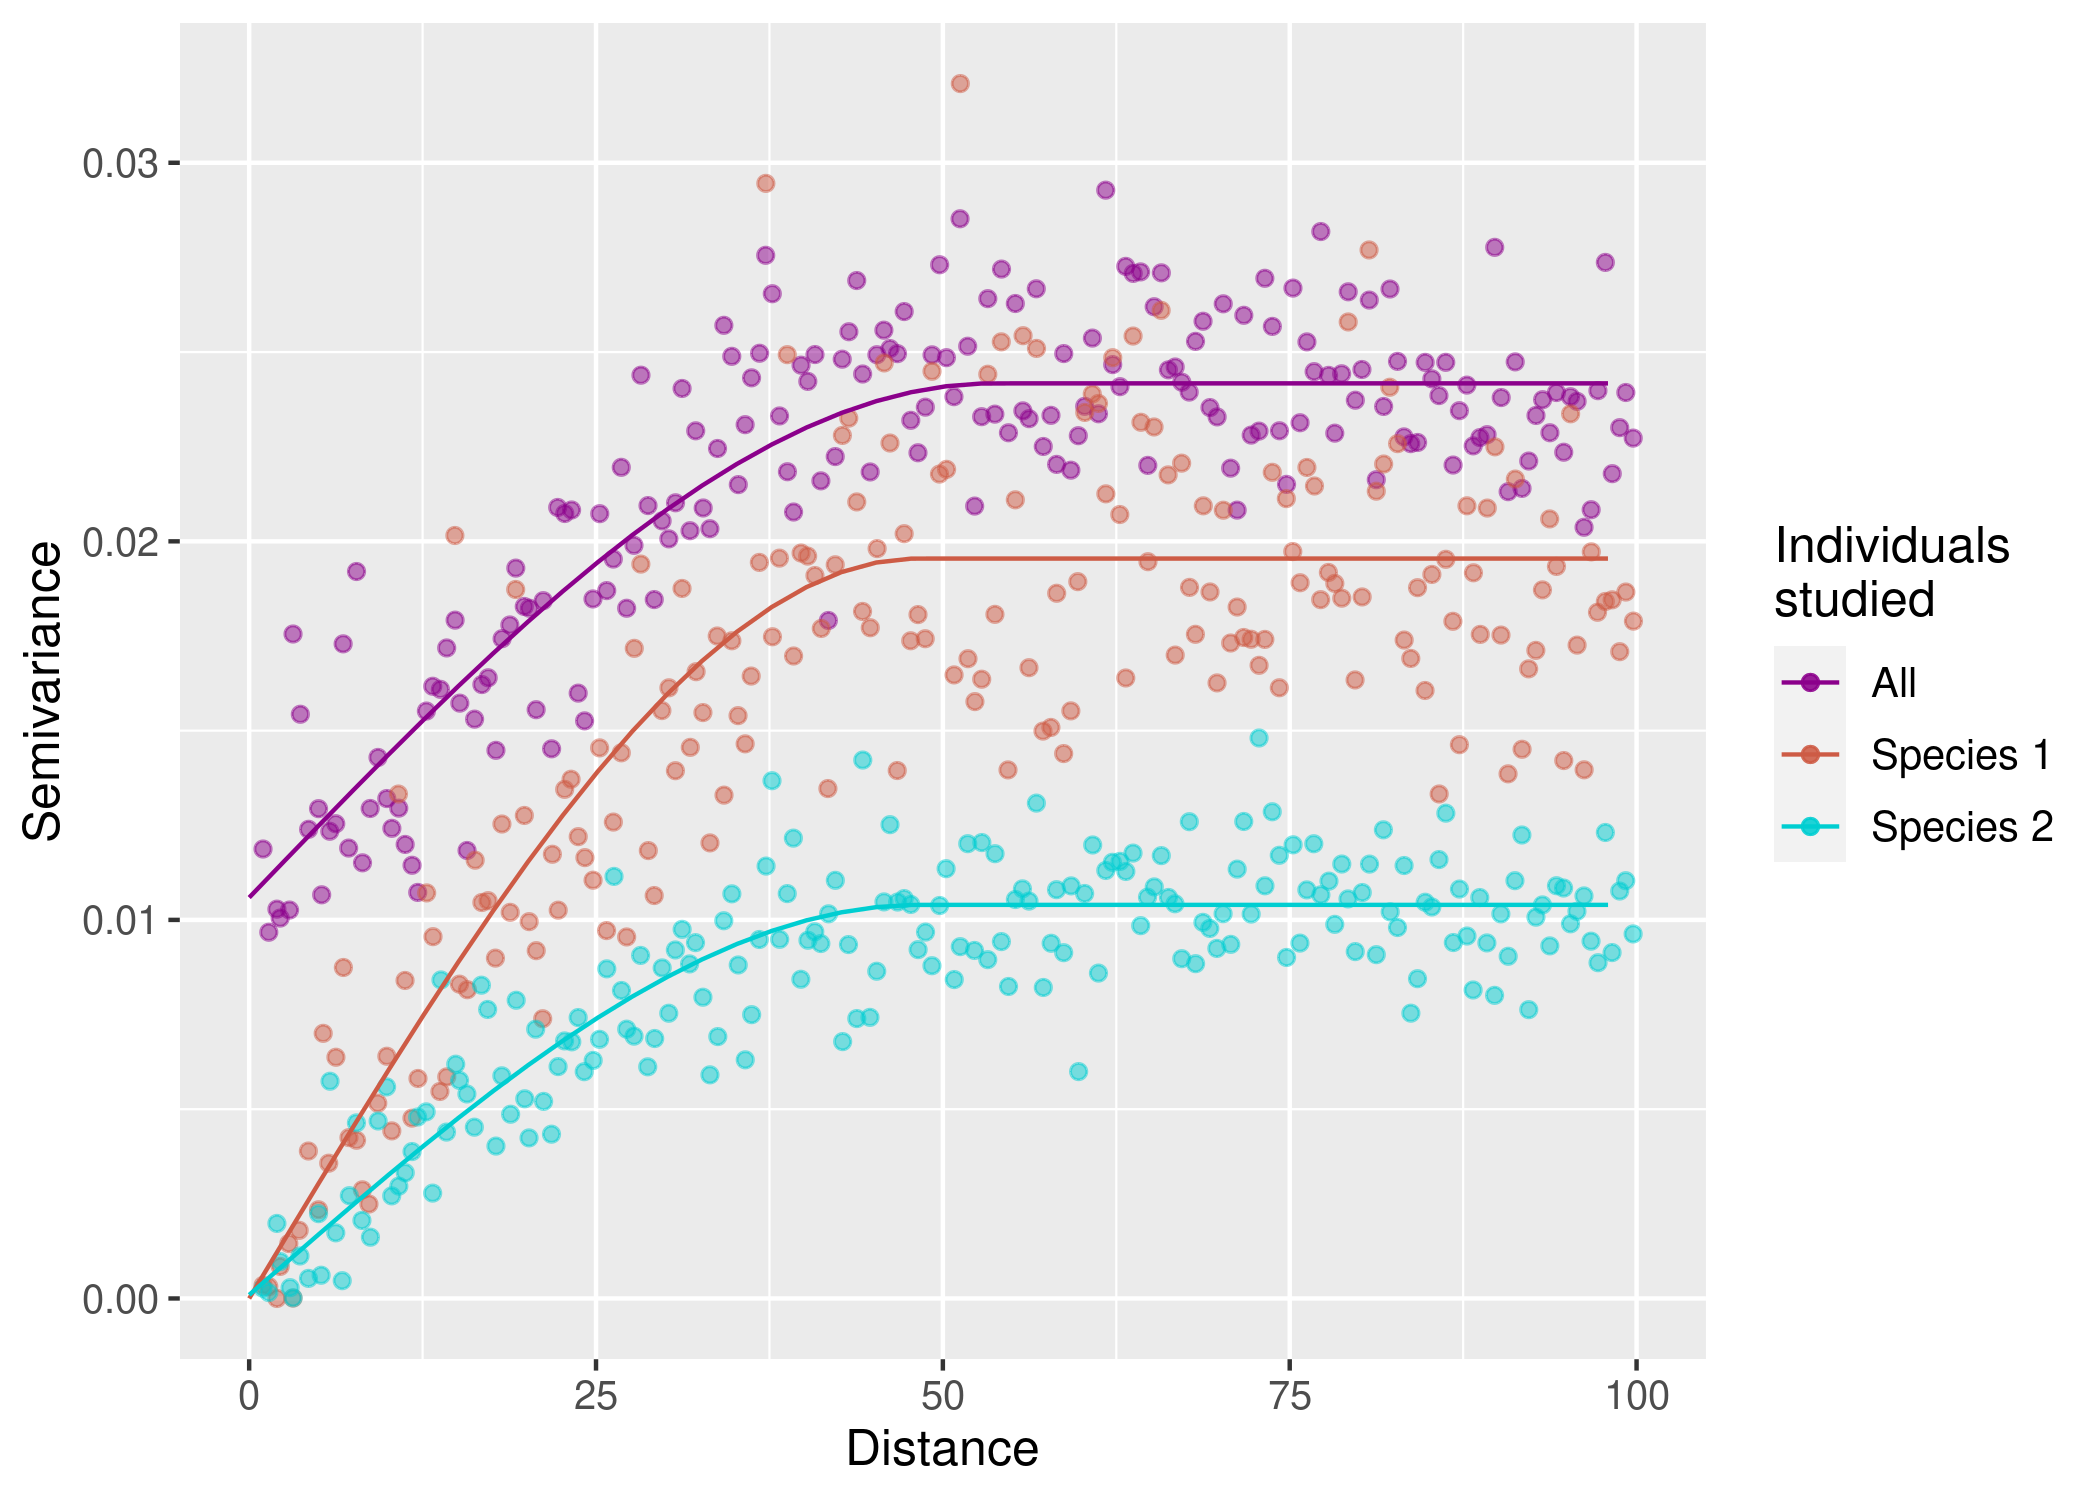
\includegraphics[width=29.17in]{/home/girard-tercieux/Code/coexIV/outputs/theoretical_model/figures/Semivariograms}

As the semivariance between individuals of both species is higher than
the semivariance between conspecifics, individual growth is more similar
between conspecifics than heterospecifics. Considering growth as a proxy
of fitness, and linking fitness to competition, we argue that in a
Lotka-Volterra model, this would translate into
\(\alpha_{i,i} > \alpha_{i,j}\), the main condition for stable
coexistence.

Therefore, stable coexistence is possible even with high intraspecific
variability, especially when this variability is not intrinsic but due
to environmental heterogeneity that is structured in space.

\end{document}
